\documentclass[10pt]{beamer}
%\mode<presentation>{}

\usepackage{media9}
\usepackage{amssymb,amsmath,amsthm,enumerate}
\usepackage[utf8]{inputenc}
\usepackage{array}
\usepackage[parfill]{parskip}
\usepackage{graphicx}
\usepackage{caption}
\usepackage{subcaption}
\usepackage{bm}
\usepackage{amsfonts,amscd}
\usepackage[]{units}
\usepackage{listings}
\usepackage{multicol}
\usepackage{multirow}
\usepackage{tcolorbox}
\usepackage{physics}
\newcommand{\R}{\mathbb{R}}
\usepackage{algorithm2e}
\usepackage{lastpage}
\usepackage{fancyhdr}
\pagestyle{fancy}
\fancyfoot[C]{Page \thepage\ of \pageref{LastPage}}

% Enable colored hyperlinks
\hypersetup{colorlinks=true}

% The following three lines are for crossmarks & checkmarks
\usepackage{pifont}% http://ctan.org/pkg/pifont
\newcommand{\cmark}{\ding{51}}%
\newcommand{\xmark}{\ding{55}}%

% Numbered captions of tables, pictures, etc.
\setbeamertemplate{caption}[numbered]

%\usepackage[superscript,biblabel]{cite}
\usepackage{algorithm2e}
\renewcommand{\thealgocf}{}

% Bibliography settings
\usepackage[style=ieee]{biblatex}
\setbeamertemplate{bibliography item}{\insertbiblabel}
\addbibresource{references.bib}

% Glossary entries
\usepackage[acronym]{glossaries}
\newacronym{ML}{ML}{machine learning}



\theoremstyle{remark}
\newtheorem*{remark}{Remark}
\theoremstyle{definition}

\newcommand{\empy}[1]{{\color{darkorange}\emph{#1}}}
\newcommand{\empr}[1]{{\color{blue}\emph{#1}}}
\newcommand{\examplebox}[2]{
\begin{tcolorbox}[colframe=darkcardinal,colback=boxgray,title=#1]
#2
\end{tcolorbox}}

\usetheme{Stanford} 
\def \i  {\item}
\def \ai {\item[] \quad \arrowbullet}
\newcommand \si[1]{\item[] \quad \bulletcolor{#1}}
\def \wi {\item[] \quad $\ \phantom{\Rightarrow}\ $}
\def \bi {\begin{itemize}\item}
\def \ei {\end{itemize}}
\def \be {\begin{equation*}}
\def \ee {\end{equation*}}
\def \bie {$\displaystyle{}
\def \eie {{\ }$}}
\def \bsie {\small$\displaystyle{}
\def \esie {{\ }$}\normalsize\selectfont}
\def \bse {\small\begin{equation*}}
\def \ese {\end{equation*}\normalsize}
\def \bfe {\footnotesize\begin{equation*}}
\def \efe {\end{equation*}\normalsize}
\renewcommand \le[1] {\\ \medskip \lefteqn{\hspace{1cm}#1} \medskip}
\def \bex {\begin{example}}
\def \eex {\end{example}}
\def \bfig {\begin{figure}}
\def \efig {\end{figure}}
\def \btheo {\begin{theorem}}
\def \etheo {\end{theorem}}
\def \bc {\begin{columns}}
\def \ec {\end{columns}}
\def \btab {\begin{tabbing}}
\def \etab {\end{tabbing}\svneg\svneg}
\newcommand \col[1]{\column{#1\linewidth}}
\def\vneg  {\vspace{-5mm}}
\def\lvneg {\vspace{-10mm}}
\def\svneg {\vspace{-2mm}}
\def\tvneg {\vspace{-1mm}}
\def\vpos  {\vspace{5mm}}
\def\lvpos {\vspace{10mm}}
\def\svpos {\vspace{2mm}}
\def\tvpos {\vspace{1mm}}
\def\hneg  {\hspace{-5mm}}
\def\lhneg {\hspace{-10mm}}
\def\shneg {\hspace{-2mm}}
\def\thneg {\hspace{-1mm}}
\def\hpos  {\hspace{5mm}}
\def\lhpos {\hspace{10mm}}
\def\shpos {\hspace{2mm}}

\logo{
\includegraphics[height=0.4in]{./style_files/kaust_academy_logo.png}}

% commands to relax beamer and subfig conflicts
% see here: https://tex.stackexchange.com/questions/426088/texlive-pretest-2018-beamer-and-subfig-collide
\makeatletter
\let\@@magyar@captionfix\relax
\makeatother

\title[Computer Vision]{Computer Vision}
%\subtitle{Subtitle Of Presentation}

%\beamertemplatenavigationsymbolsempty

\begin{document}

\author[KAUST Academy]{
	\begin{tabular}{c} 
	\Large
	Naeemullah Khan\\
    \footnotesize \href{mailto:naeemullah.khan@kaust.edu.sa}{naeemullah.khan@kaust.edu.sa}
\end{tabular}
\vspace{-4ex}}

\institute{
	\vskip 20pt
	\begin{figure}
		\centering
		\begin{subfigure}[t]{0.5\textwidth}
			\centering
			
\includegraphics[height=0.5in]{./style_files/kaust_logo.png}
		\end{subfigure}
% 		~ 
% 		\begin{subfigure}[t]{0.5\textwidth}
% 			\centering
% 			
\includegraphics[height=0.33in]{./style_files/kaust_academy_logo.png}
% 		\end{subfigure}
	\end{figure}
	\vskip 20pt
	KAUST Academy \\
	King Abdullah University of Science and Technology\\
	\vskip 3pt
}

% \date{June 15, 2020}
\date{\today}

\begin{noheadline}
\begin{frame}\maketitle\end{frame}
\end{noheadline}


\setbeamertemplate{itemize items}[default]
\setbeamertemplate{itemize subitem}[circle]

\begin{frame}{Table of Contents}
\begin{enumerate}
    \item Introduction.
    \item Applications of Computer Vision.
    \item Image Representation.
    \item Convolutional Neural Network (CNN) and its Components.
    \item CNN-based Architectures (AlexNet, VGG, InceptionNet, ResNet, EfficientNet, and MobileNet).
\end{enumerate}
\end{frame}

\begin{frame}{Learning Outcomes}
\begin{itemize}
    \item Understand the basic concepts of Computer Vision and its real-world applications.
    \item Describe how images are represented and processed in a computer.
    \item Explain the fundamental building blocks of Convolutional Neural Networks (CNNs).
    \item Differentiate between popular CNN architectures (AlexNet, VGG, InceptionNet, ResNet, EfficientNet, and MobileNet) and their key innovations.
\end{itemize}
\end{frame}



\begin{frame}{Computer Vision}
\centering
Building artificial systems that process, perceive, and reason about visual data

    
\end{frame}

\begin{frame}{Computer Vision is Everywhere}
\begin{figure}
\centering
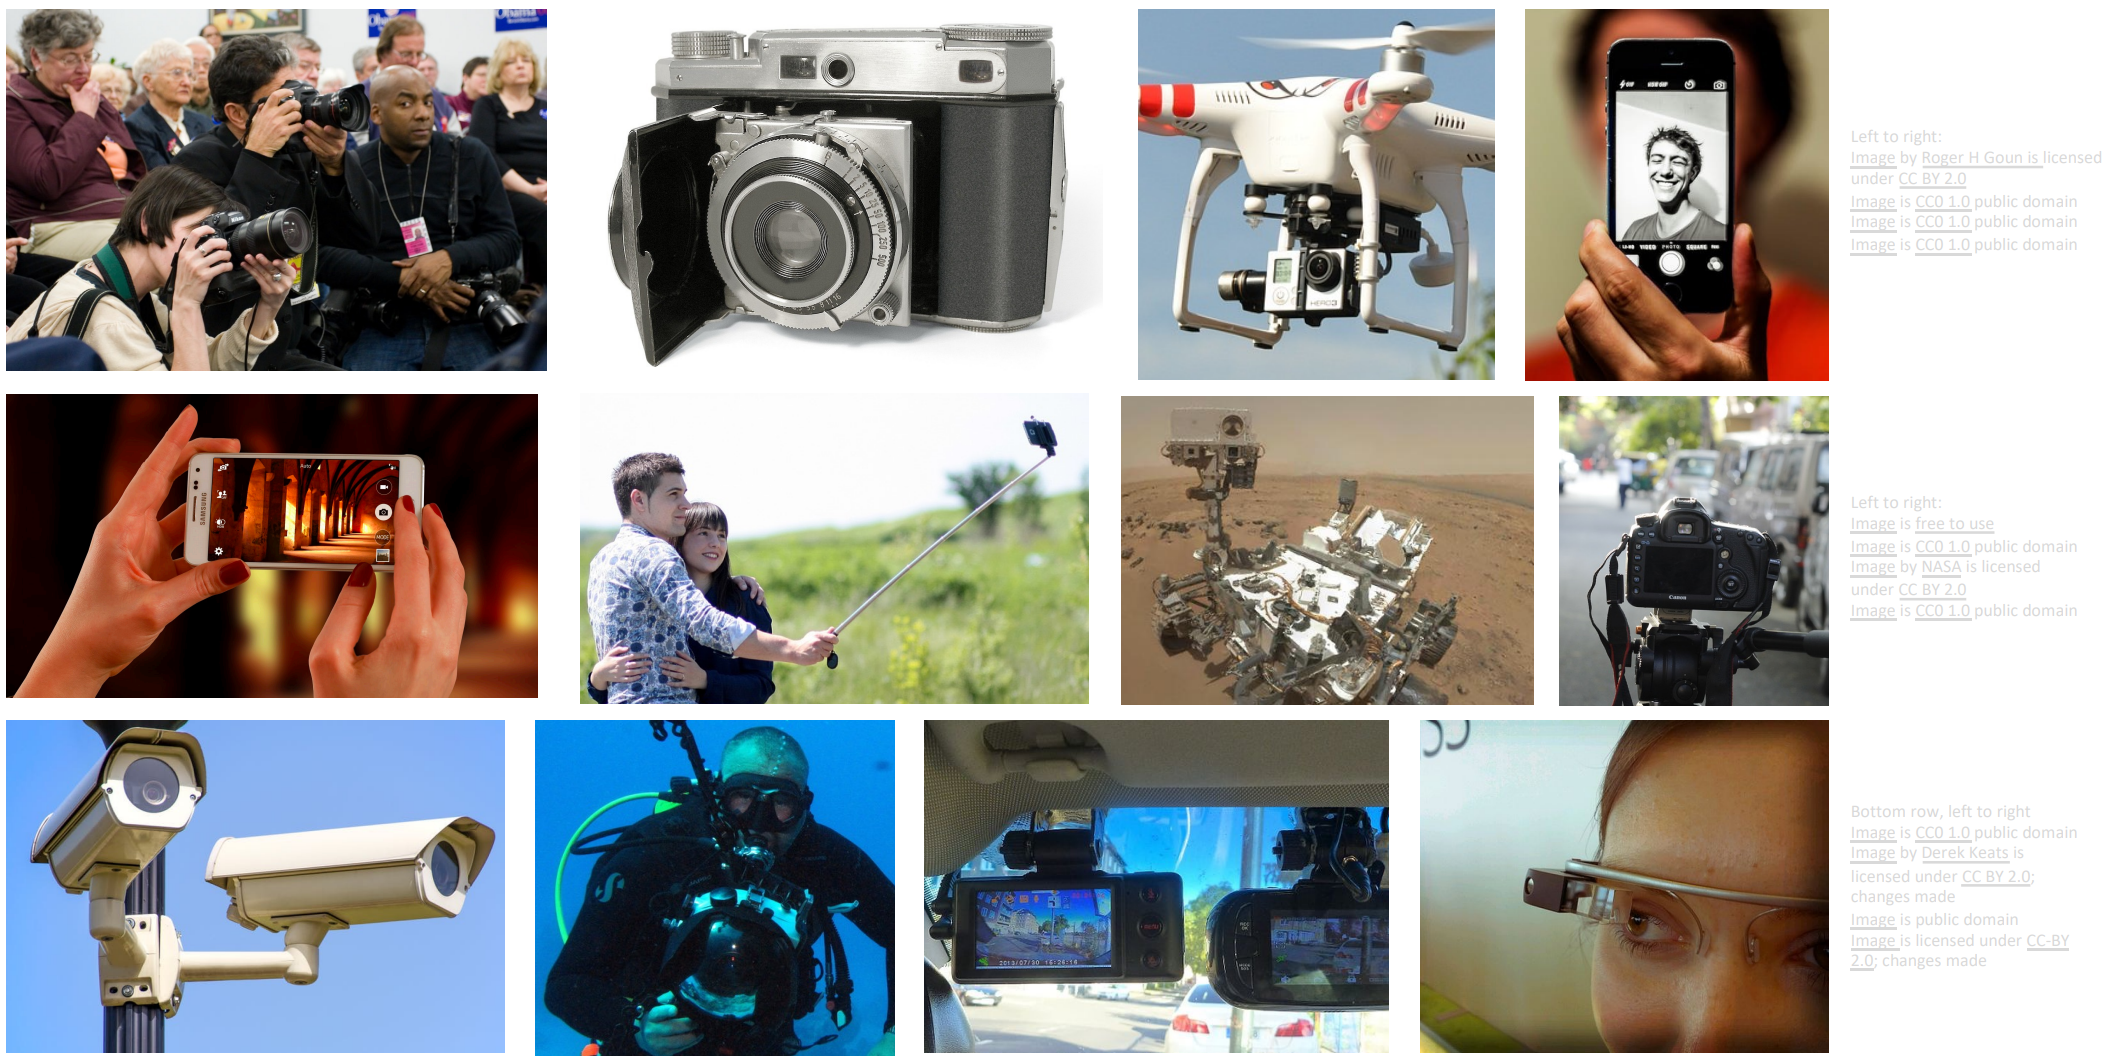
\includegraphics[width=1.0\textwidth,height=1.0\textheight,keepaspectratio]{./images/cv_1.png}
\end{figure}
    
\end{frame}

\begin{frame}[allowframebreaks]{Some Applications}
\begin{figure}
\centering
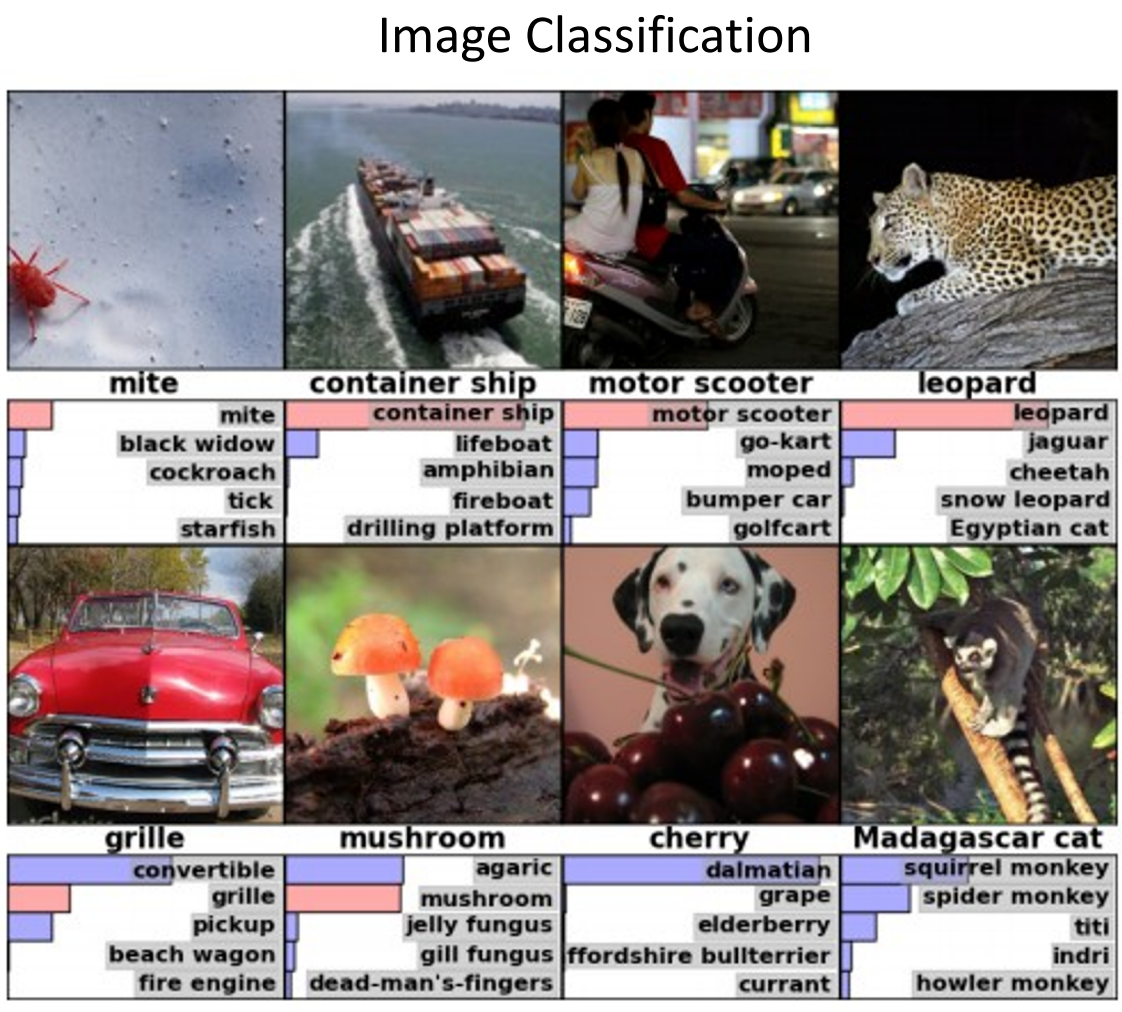
\includegraphics[width=1.0\textwidth,height=0.9\textheight,keepaspectratio]{./images/cv_2.png}
\end{figure}

\framebreak

\begin{figure}
\centering
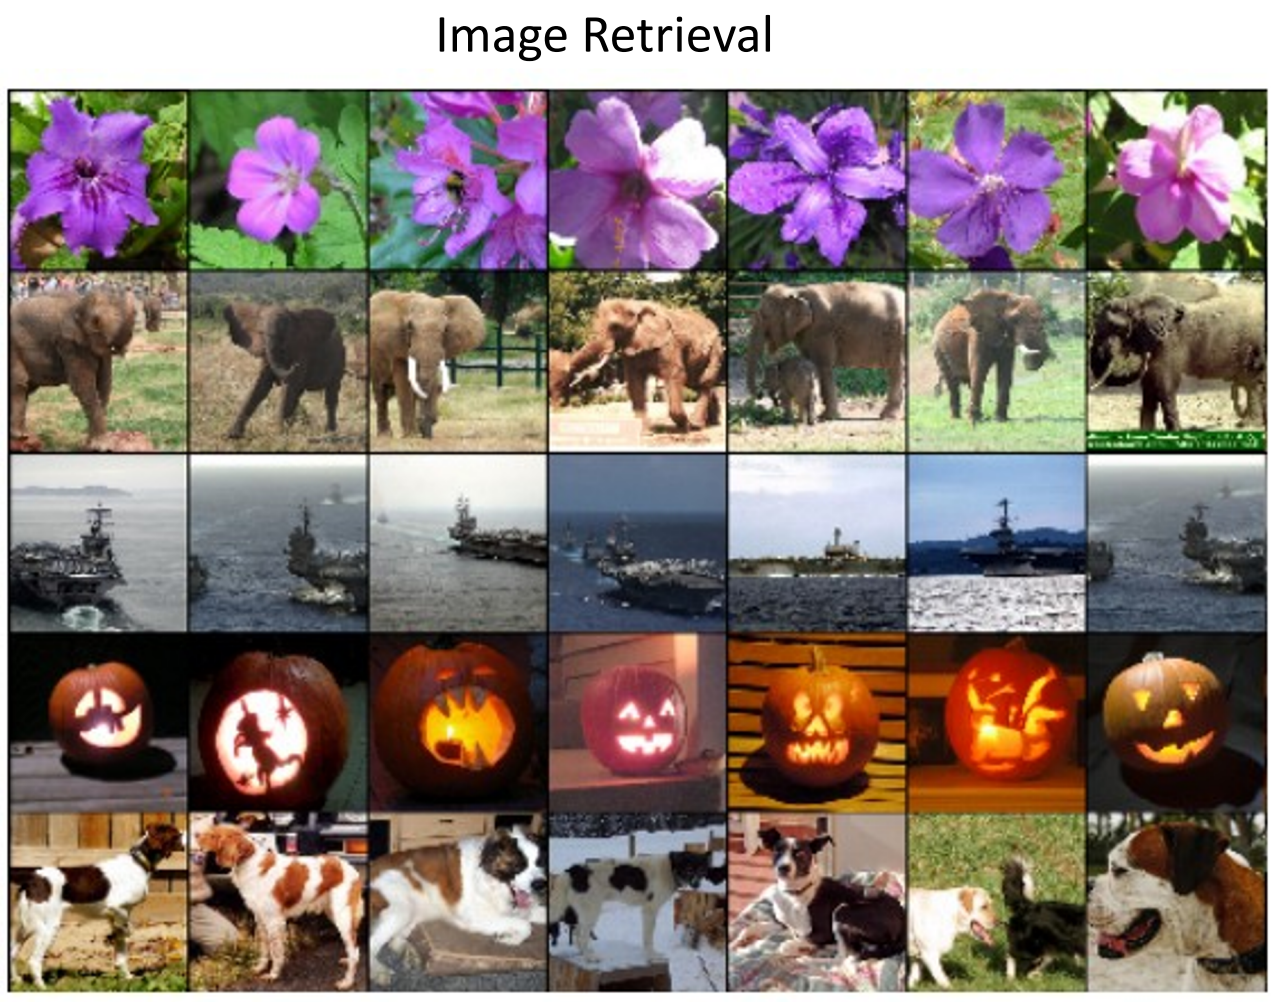
\includegraphics[width=1.0\textwidth,height=0.9\textheight,keepaspectratio]{./images/cv_3.png}
\end{figure}

\framebreak

\begin{figure}
\centering
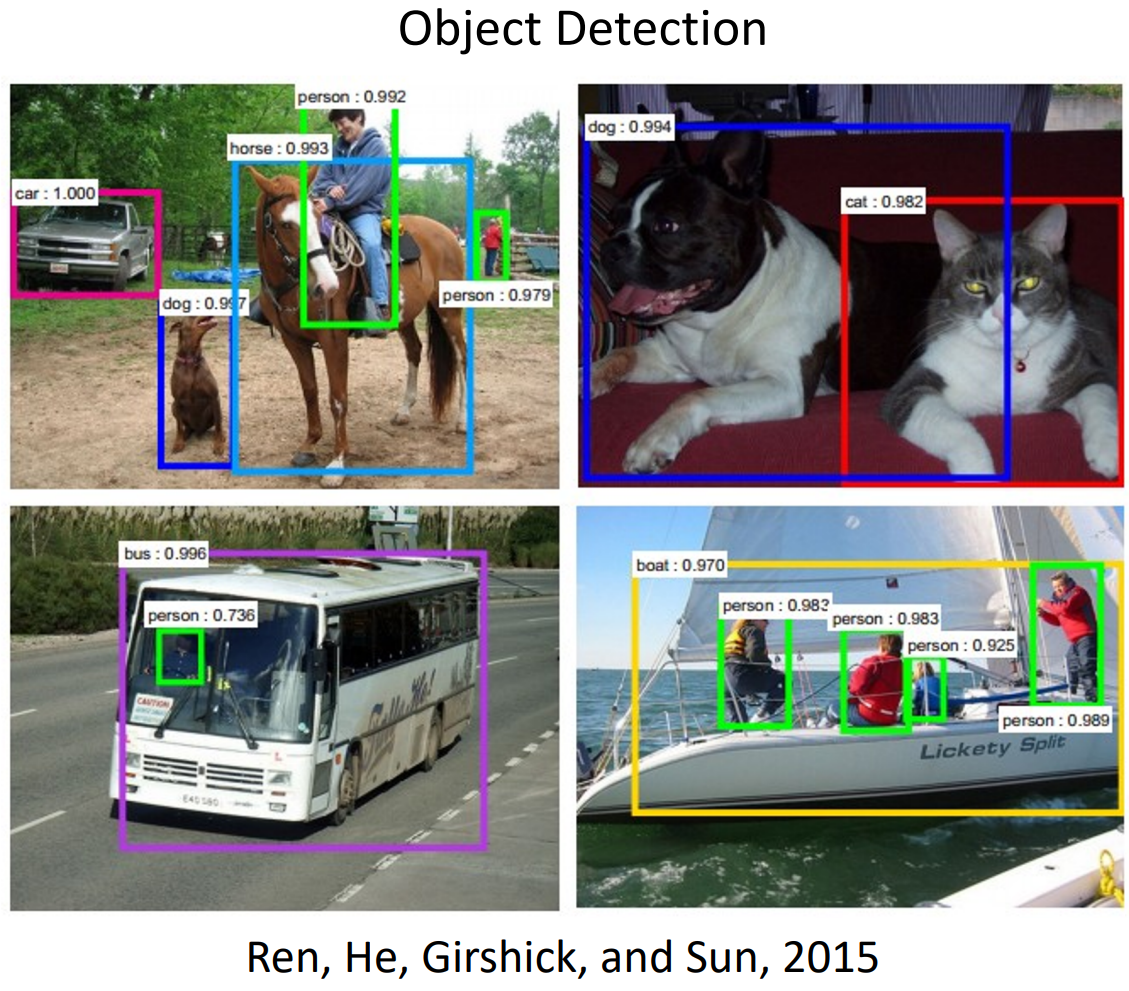
\includegraphics[width=1.0\textwidth,height=0.9\textheight,keepaspectratio]{./images/cv_4.png}
\end{figure}

\framebreak

\begin{figure}
\centering
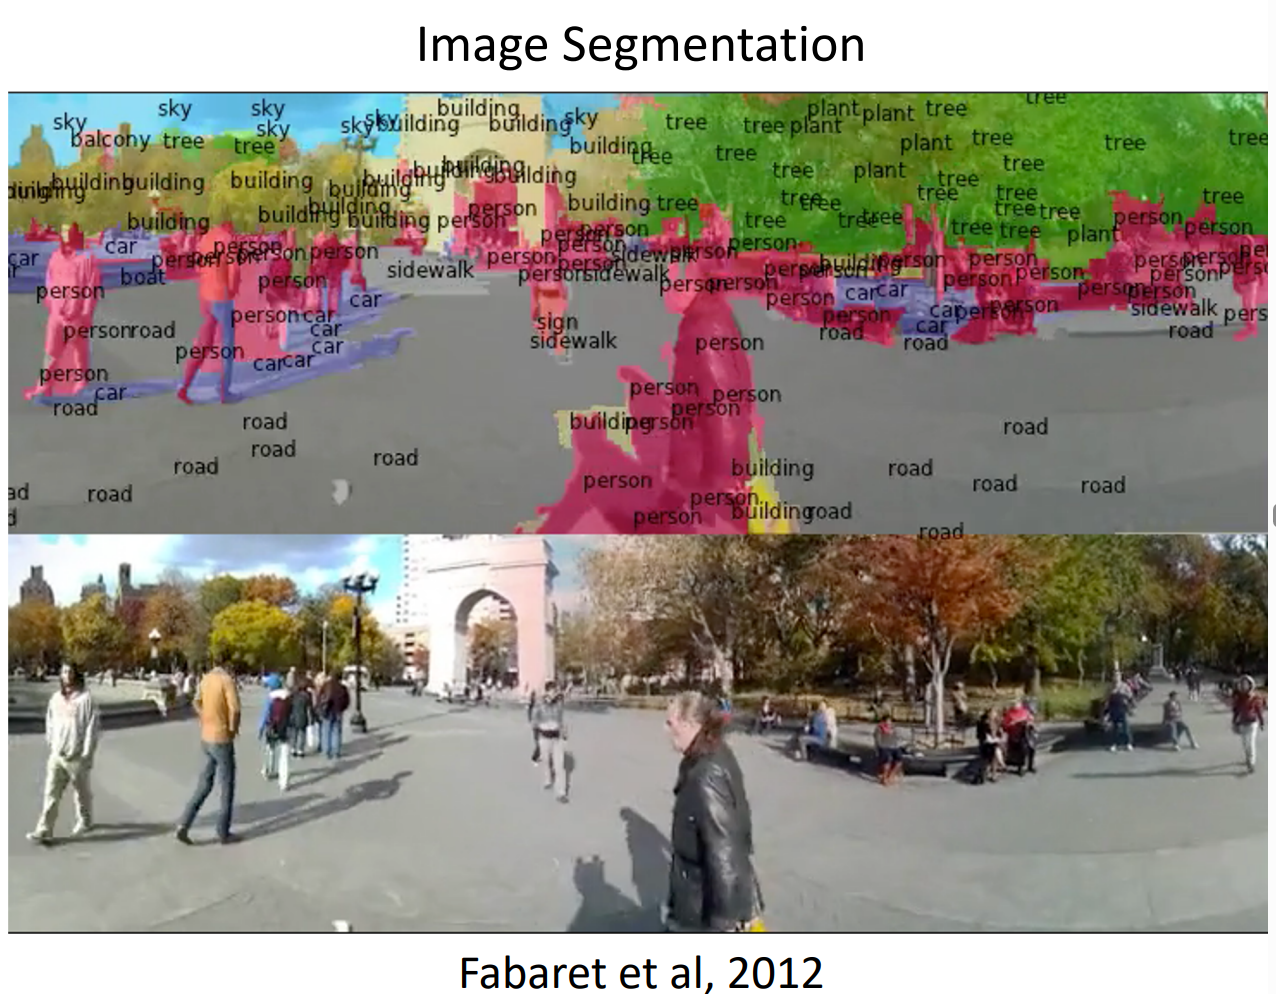
\includegraphics[width=1.0\textwidth,height=0.9\textheight,keepaspectratio]{./images/cv_5.png}
\end{figure}

\framebreak

\begin{figure}
\centering
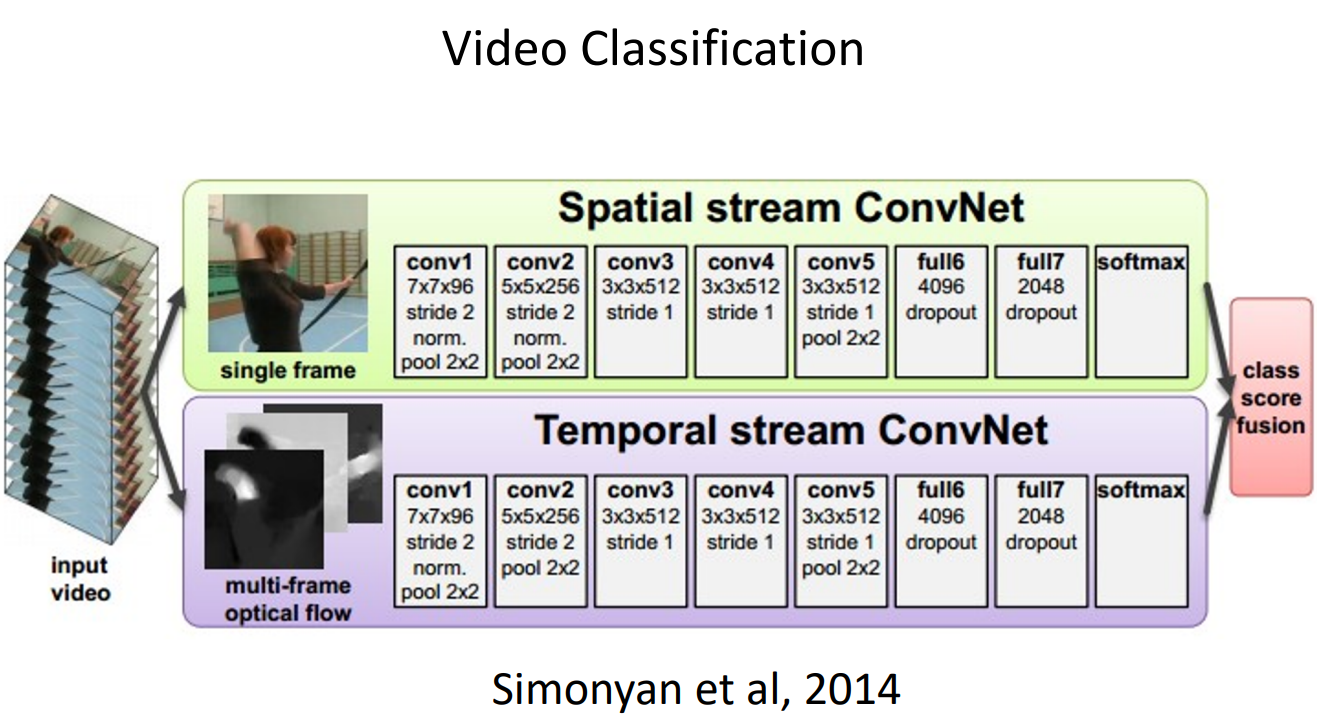
\includegraphics[width=1.0\textwidth,height=0.9\textheight,keepaspectratio]{./images/cv_6.png}
\end{figure}


\framebreak

\begin{figure}
\centering
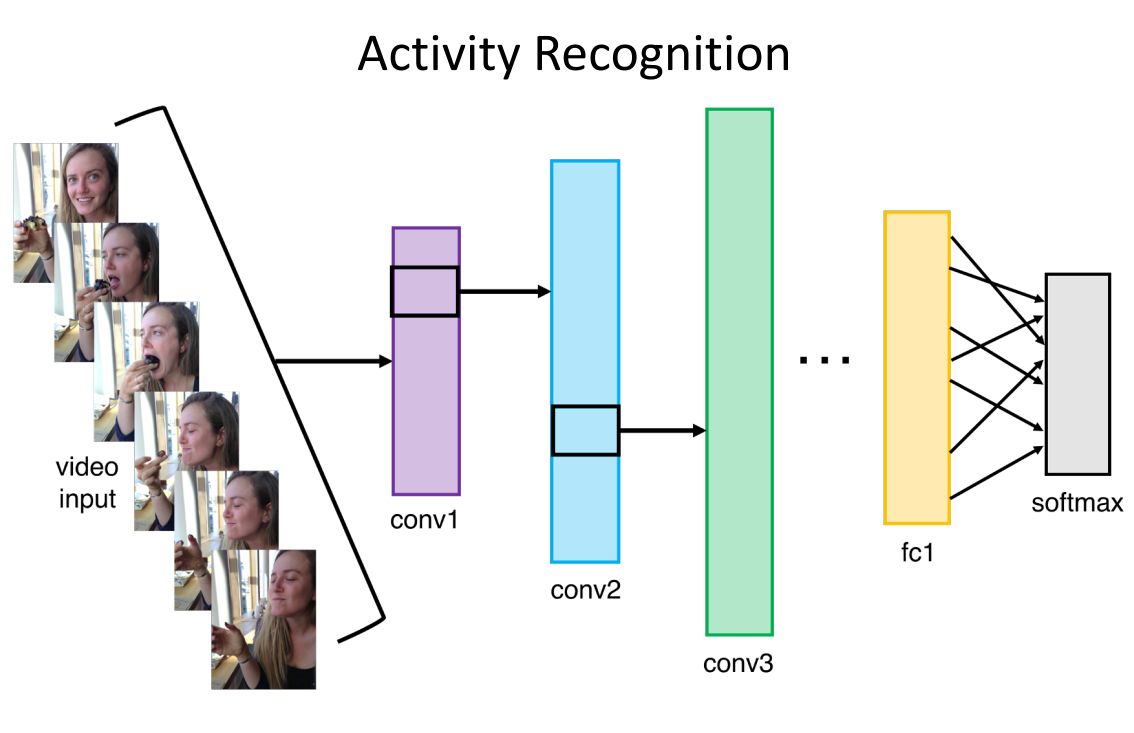
\includegraphics[width=1.0\textwidth,height=0.9\textheight,keepaspectratio]{./images/cv_7.png}
\end{figure}

\framebreak

\begin{figure}
\centering
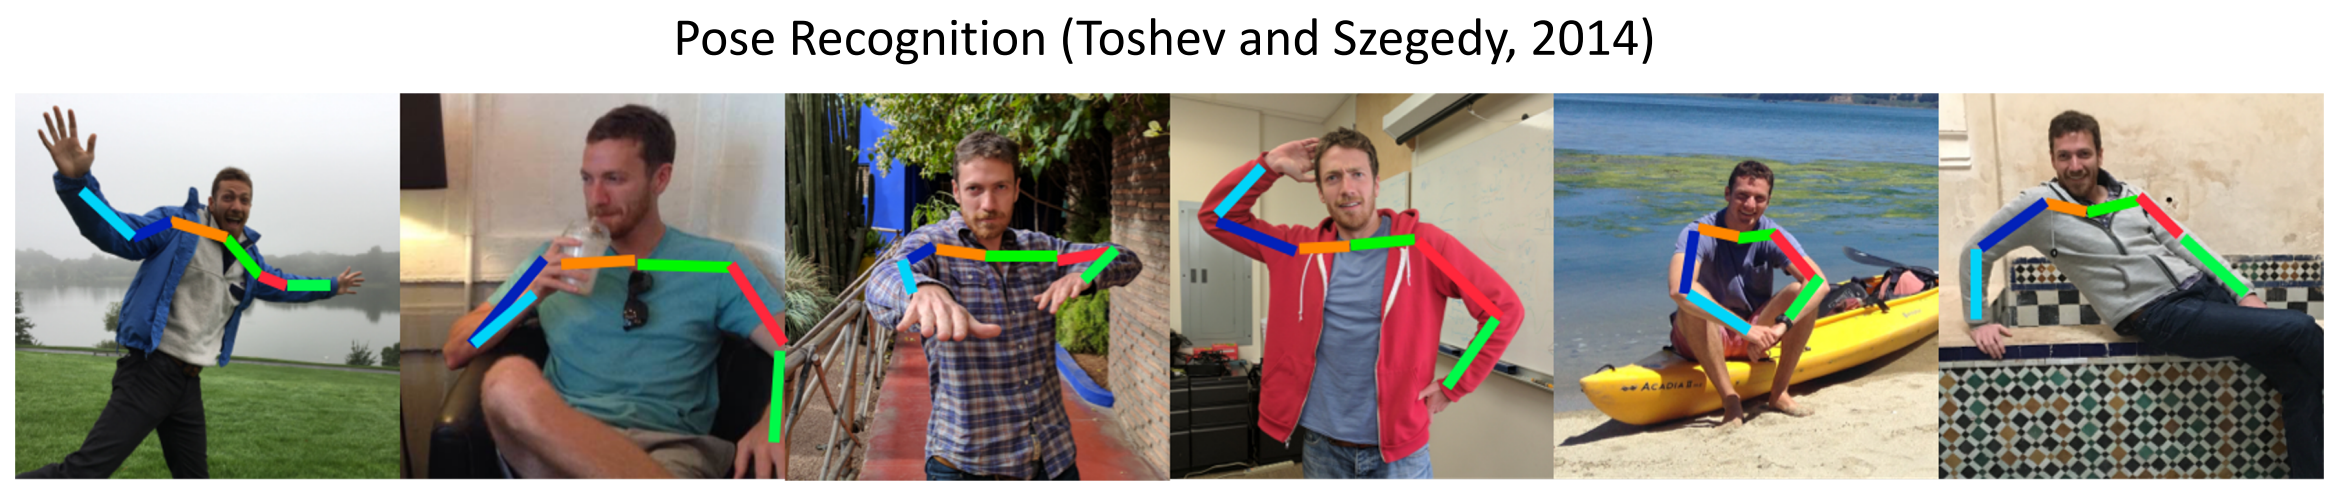
\includegraphics[width=1.0\textwidth,height=0.9\textheight,keepaspectratio]{./images/cv_8.png}
\end{figure}

\framebreak

\begin{figure}
\centering
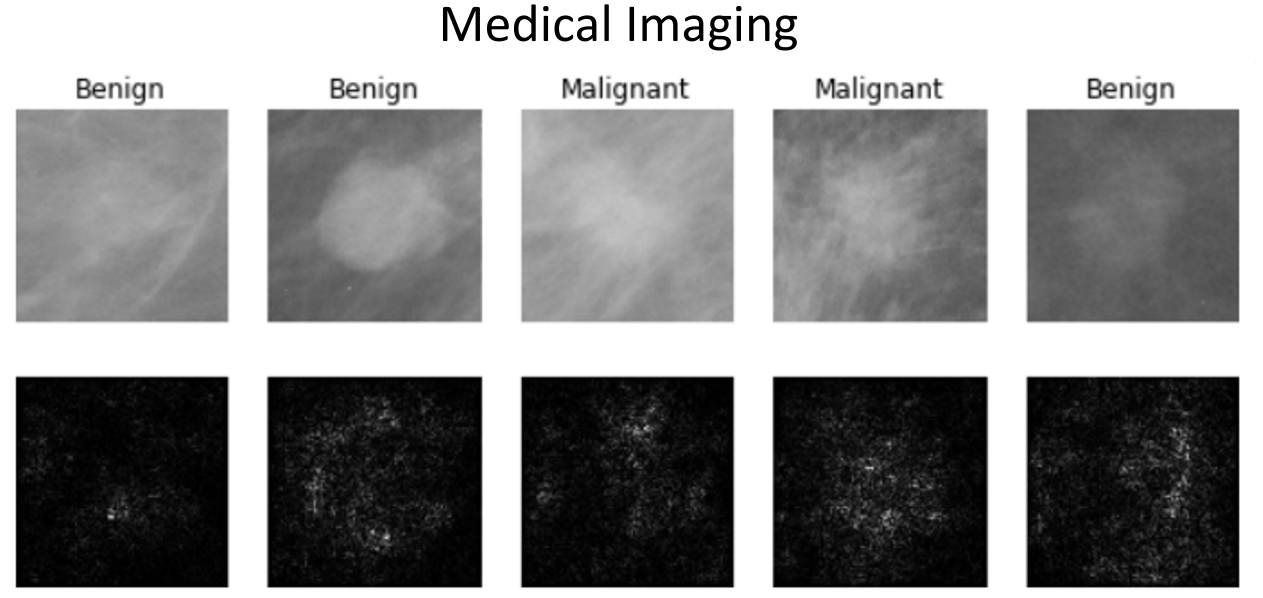
\includegraphics[width=1.0\textwidth,height=0.9\textheight,keepaspectratio]{./images/cv_9.png}
\end{figure}

\framebreak

\begin{figure}
\centering
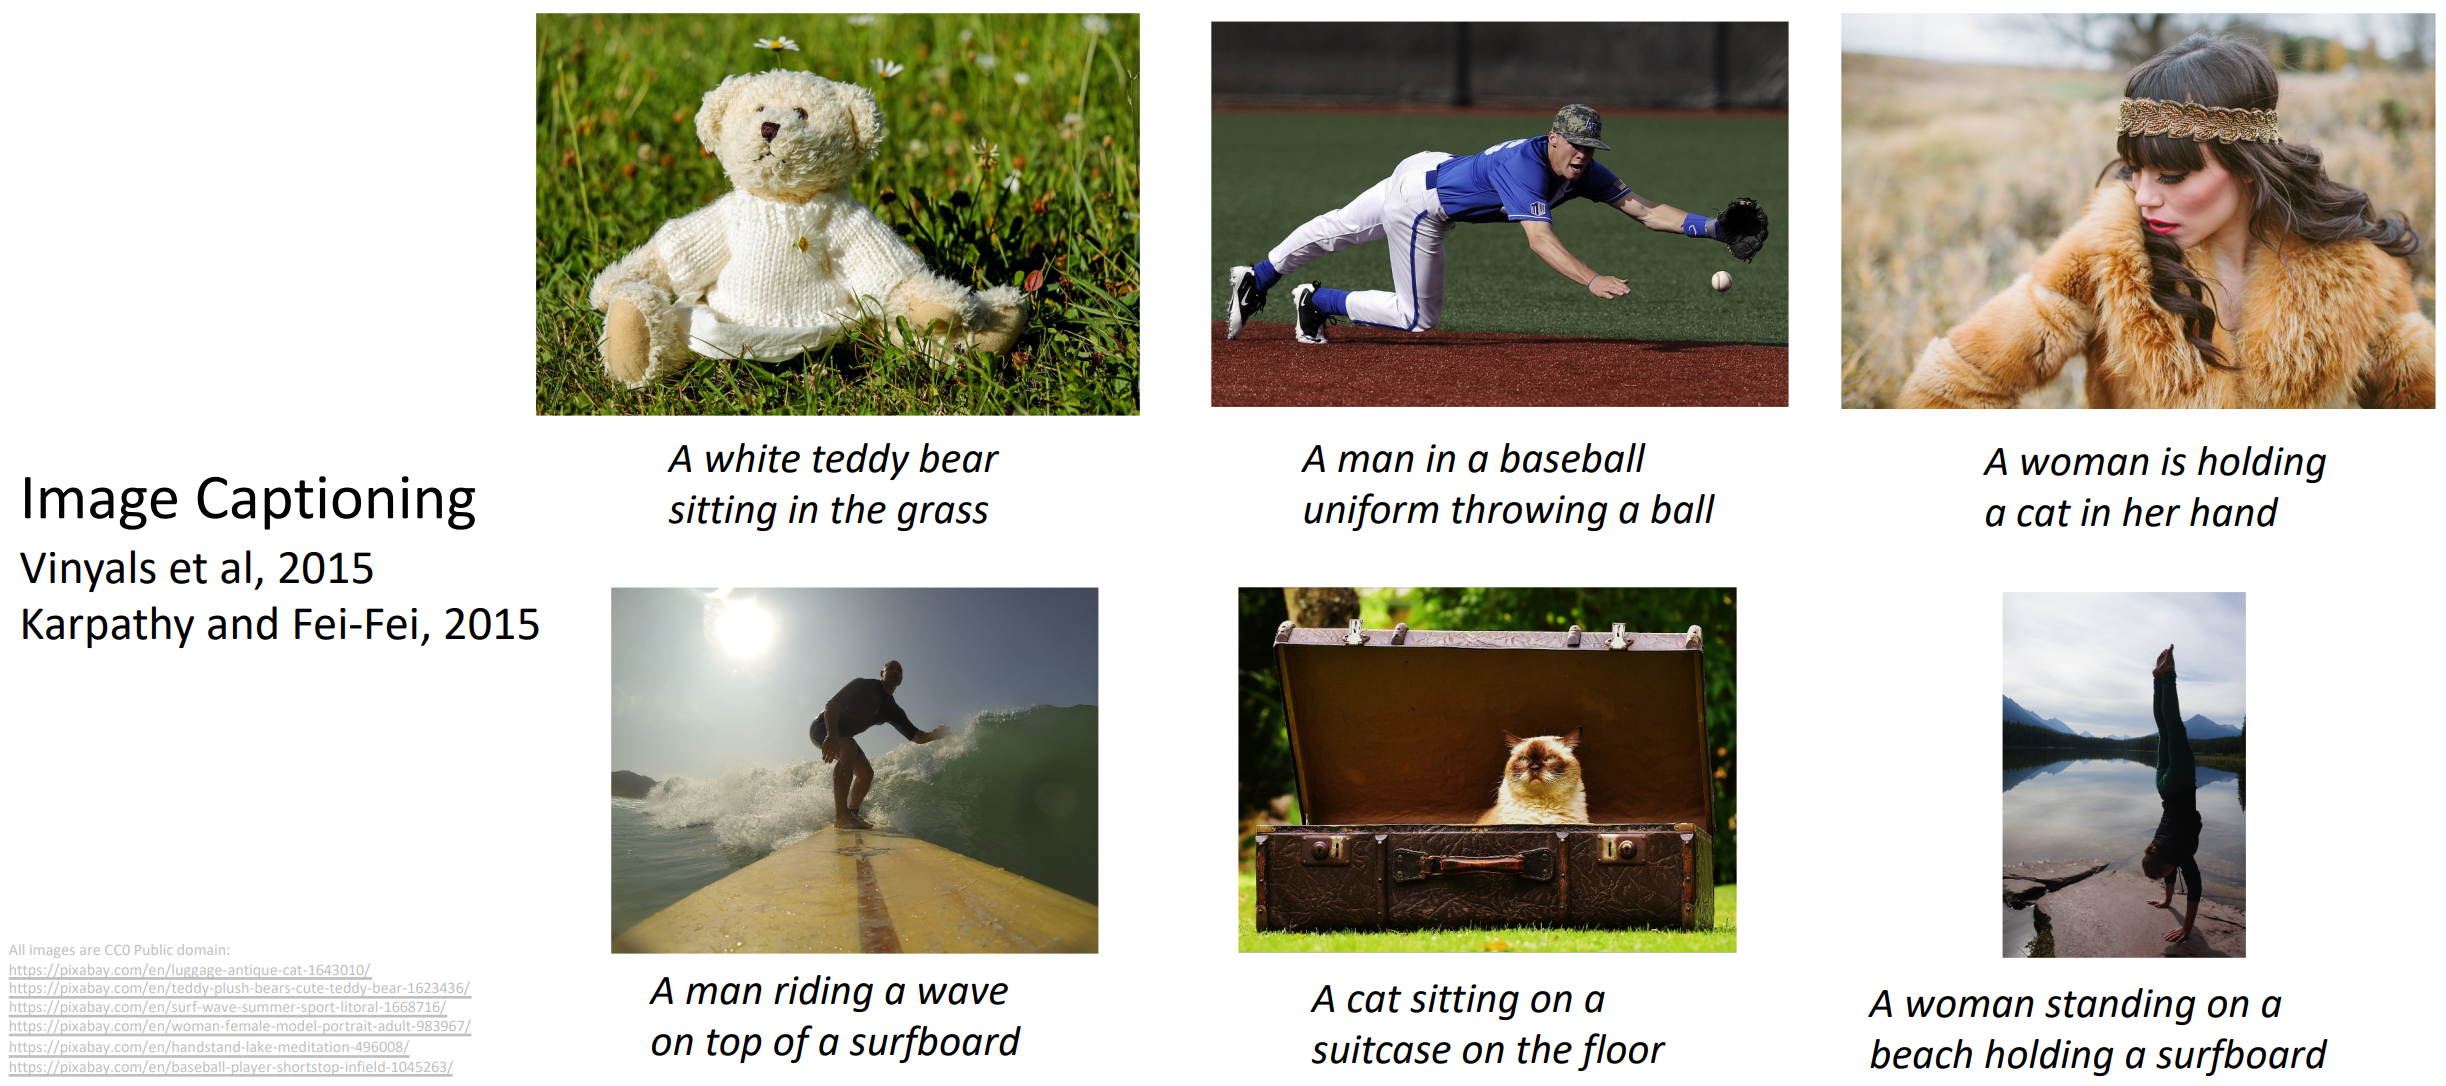
\includegraphics[width=1.0\textwidth,height=0.9\textheight,keepaspectratio]{./images/cv_10.png}
\end{figure}

\framebreak

\centering
Image Generation
\begin{figure}
\centering
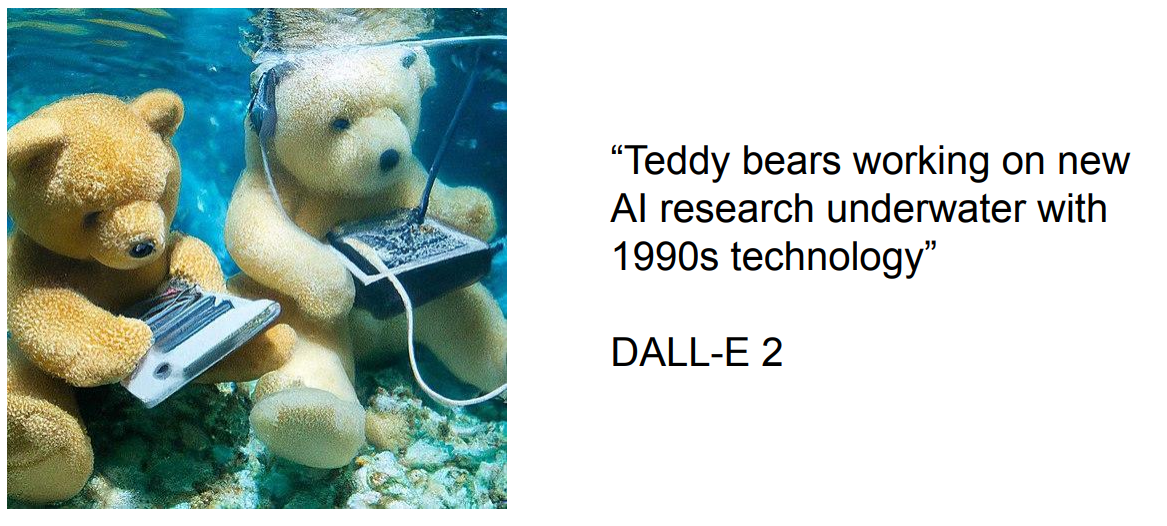
\includegraphics[width=1.0\textwidth,height=0.9\textheight,keepaspectratio]{./images/cv_11.png}
\end{figure}

\framebreak

\begin{figure}
\centering
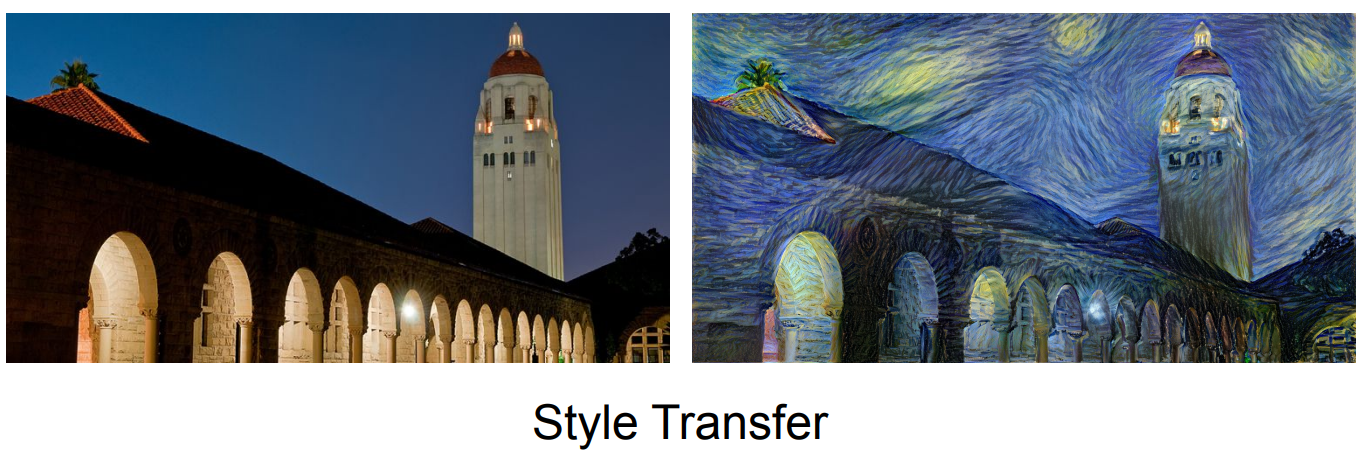
\includegraphics[width=1.0\textwidth,height=0.9\textheight,keepaspectratio]{./images/cv_12.png}
\end{figure}

\framebreak

\centering
3D Vision
\begin{figure}
\centering
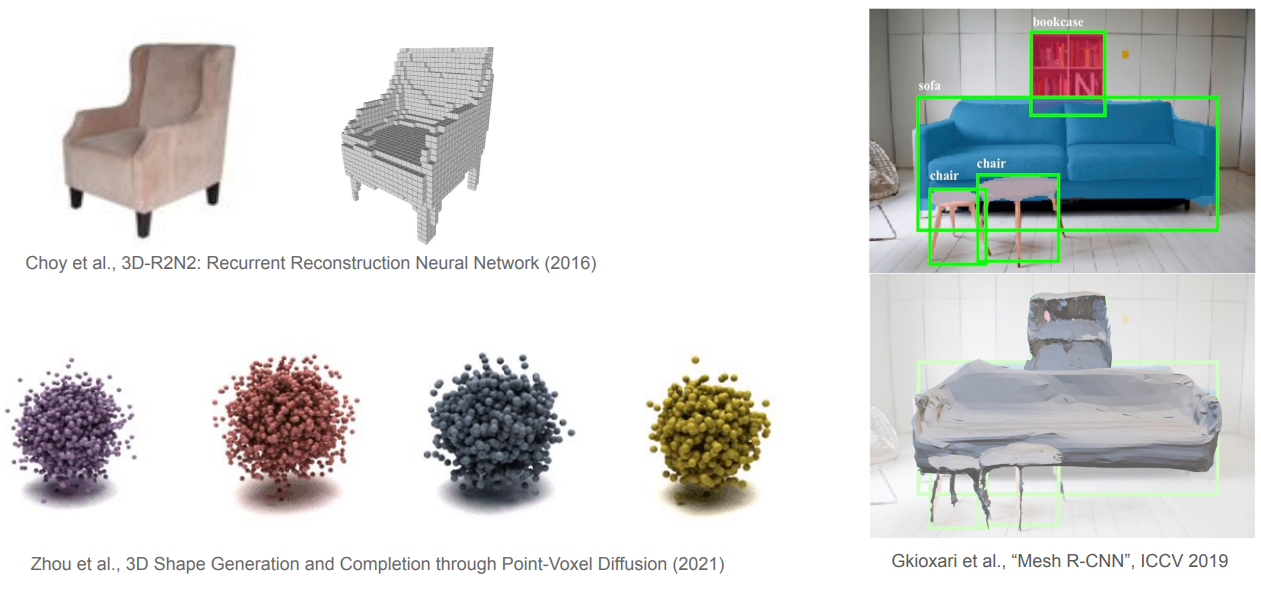
\includegraphics[width=1.0\textwidth,height=0.9\textheight,keepaspectratio]{./images/cv_13.png}
\end{figure}
    
\end{frame}


\begin{frame}{How to represent an image?}
\begin{itemize}
    \item Images are represented as Matrices with elements in $[0,255]$
    \item Grayscale images have one channel.
\end{itemize}
\begin{figure}
\centering
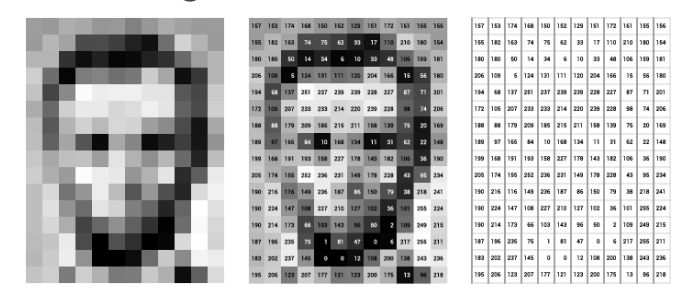
\includegraphics[width=1.0\textwidth,height=0.7\textheight,keepaspectratio]{./images/represent_image.png}
\end{figure}

\footnotetext{https://www.v7labs.com/blog/image-recognition-guide}
\end{frame}

\begin{frame}{How to represent an image?}
\begin{itemize}

    \item RGB images have 3 channels.
\end{itemize}
\begin{figure}
\centering
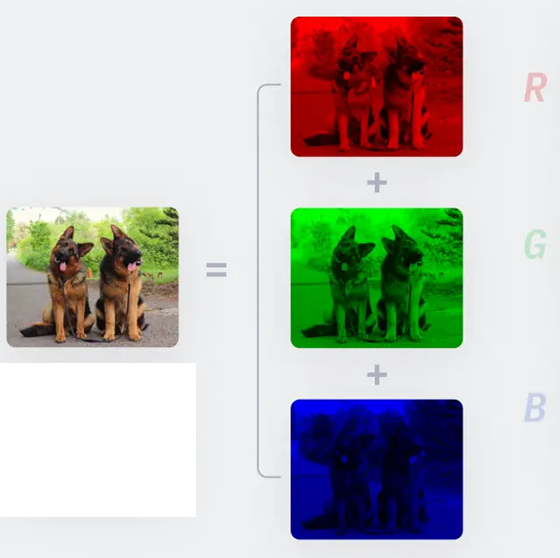
\includegraphics[width=1.5\textwidth,height=0.7\textheight,keepaspectratio]{./images/RGB.png}
\end{figure}
\end{frame}

\begin{frame}{How can we build vision models?}
\begin{itemize}
    \item So far, we’ve worked with tabular data, where each sample consists of structured features. We processed this data using Fully Connected Neural Networks.

\end{itemize}
\begin{figure}
\centering
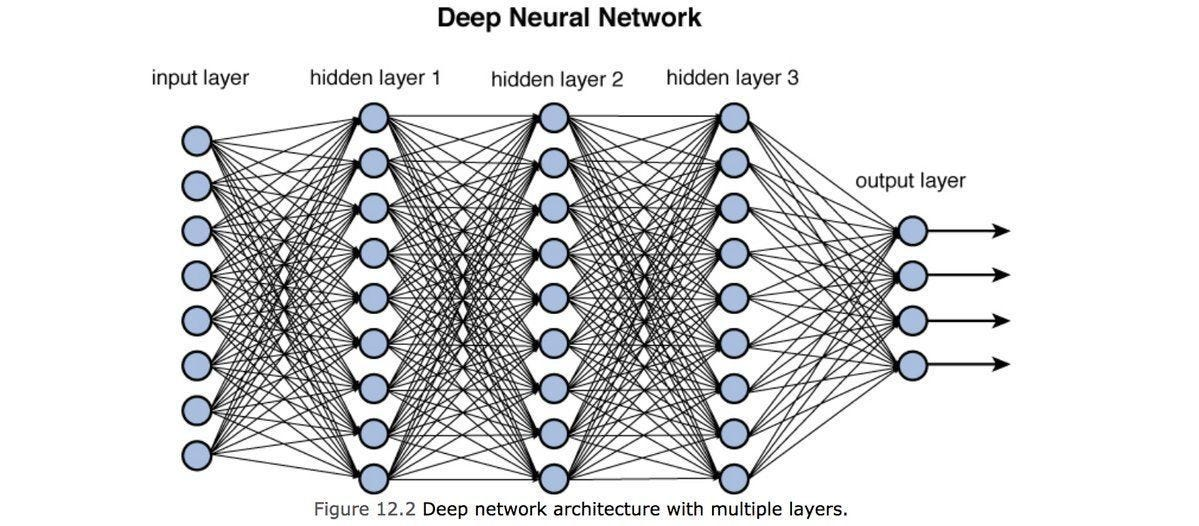
\includegraphics[width=1.0\textwidth,height=1.0\textheight,keepaspectratio]{./images/nn.jpg}
\end{figure}
\begin{itemize}
    \item But can we apply the same approach to images?
\end{itemize}

\end{frame}

\begin{frame}{How can we build vision models?}
\begin{itemize}
    \item Let's try.
\end{itemize}
\end{frame}

\begin{frame}{How can we build vision models?}
\begin{itemize}
    \item Let's consider each pixel as a feature.
\end{itemize}

\begin{figure}
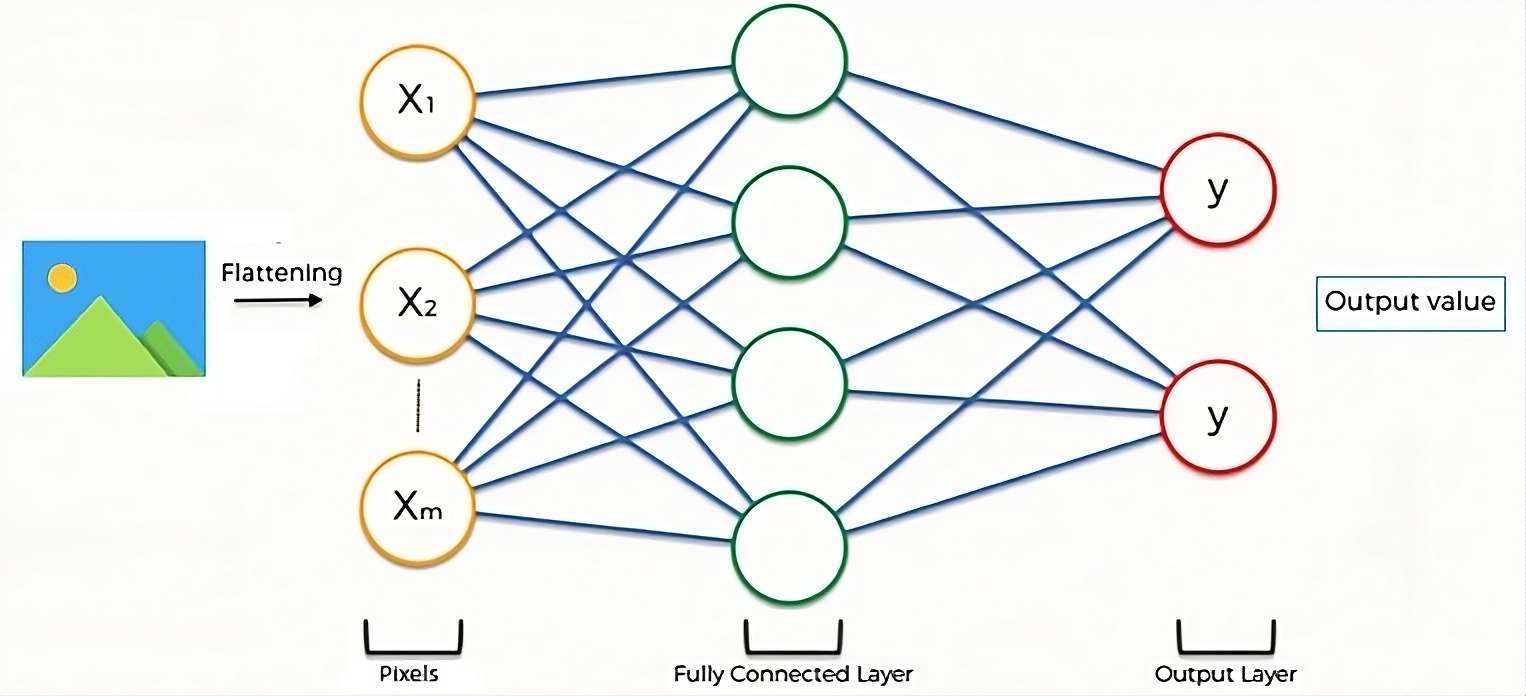
\includegraphics[width=1.0\textwidth,height=1.0\textheight,keepaspectratio]{./images/images_nn.png}
\end{figure}
\begin{itemize}
    \item This should work! But...
\end{itemize}
\end{frame}



\begin{frame}[allowframebreaks]{Drawbacks of Fully-Connected Neural Networks}
\begin{itemize}
    \item The number of trainable parameters becomes extremely large
\end{itemize}

\begin{figure}
\centering
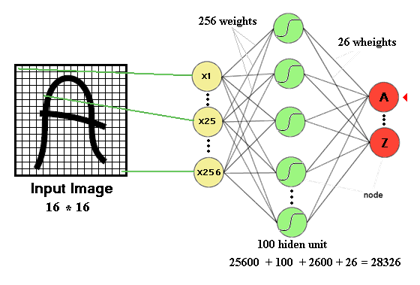
\includegraphics[width=1.0\textwidth,height=0.8\textheight,keepaspectratio]{./images/nn_2.png}
\end{figure}




\framebreak

\begin{itemize}
    \item Little or no invariance to shifting, scaling, and other forms of distortion

    \item In other words, the Fully connected NN cannot recognize that the two images (original and shifted) represent the same object (letter "A").
\end{itemize}

\begin{figure}[ht]
\centering
% First image on the left
\begin{minipage}[t]{0.45\textwidth}
    \centering
    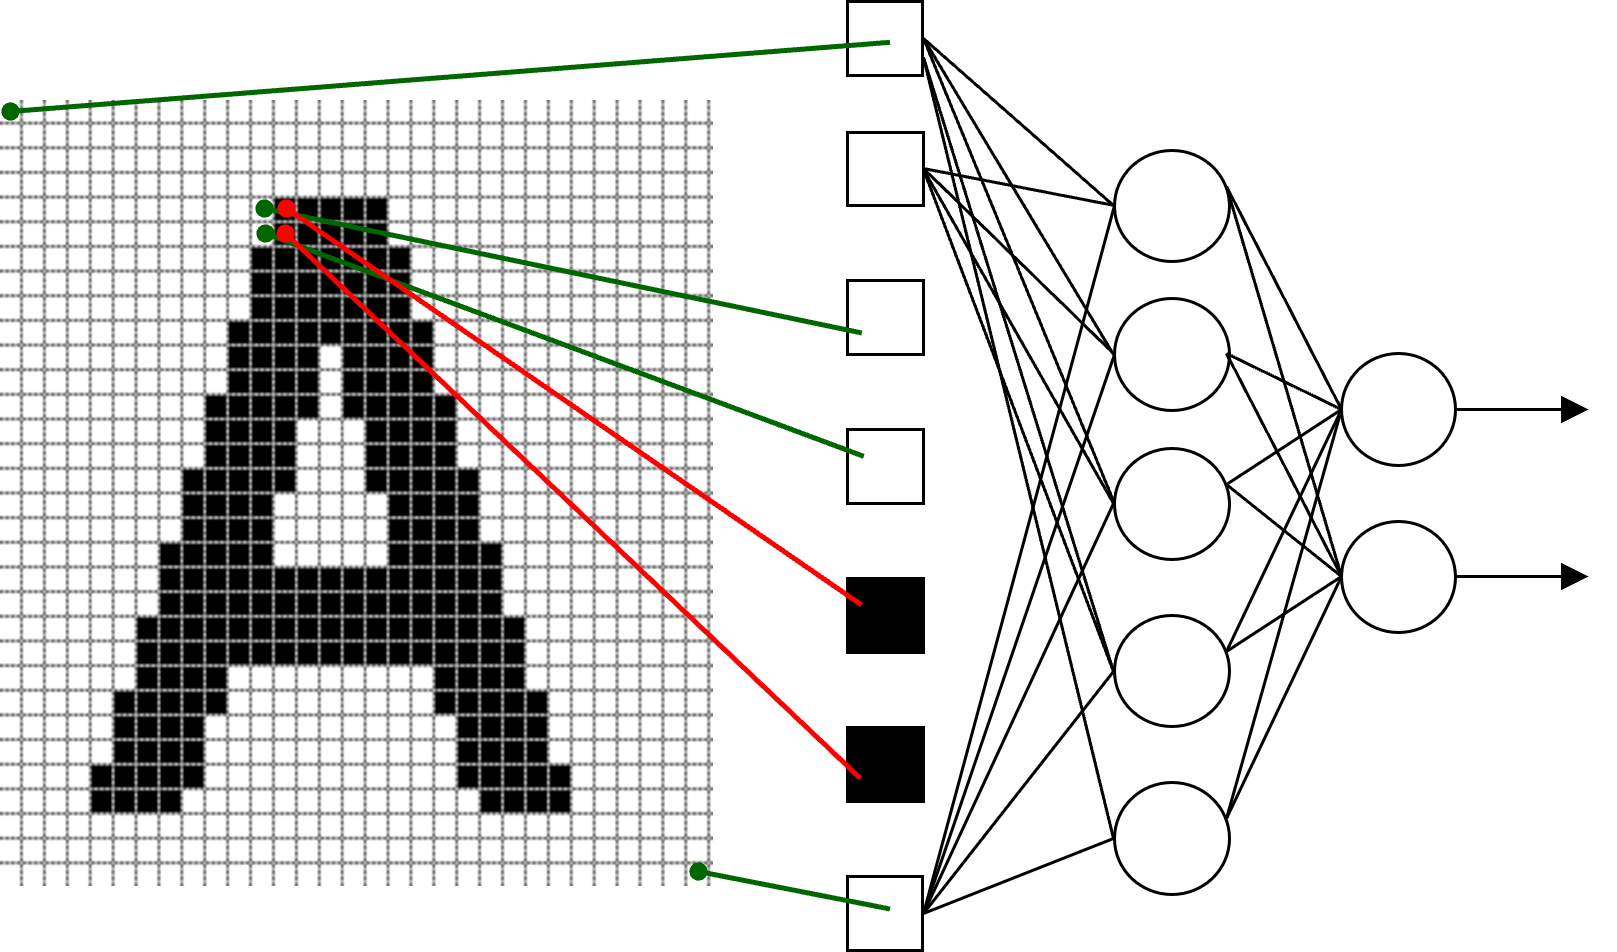
\includegraphics[width=\textwidth,height=0.7\textheight,keepaspectratio]{./images/nn_3.png}
    \caption{Original "A" character.}
    \label{fig:original_a}
\end{minipage}
\hfill
% Second image on the right
\begin{minipage}[t]{0.45\textwidth}
    \centering
    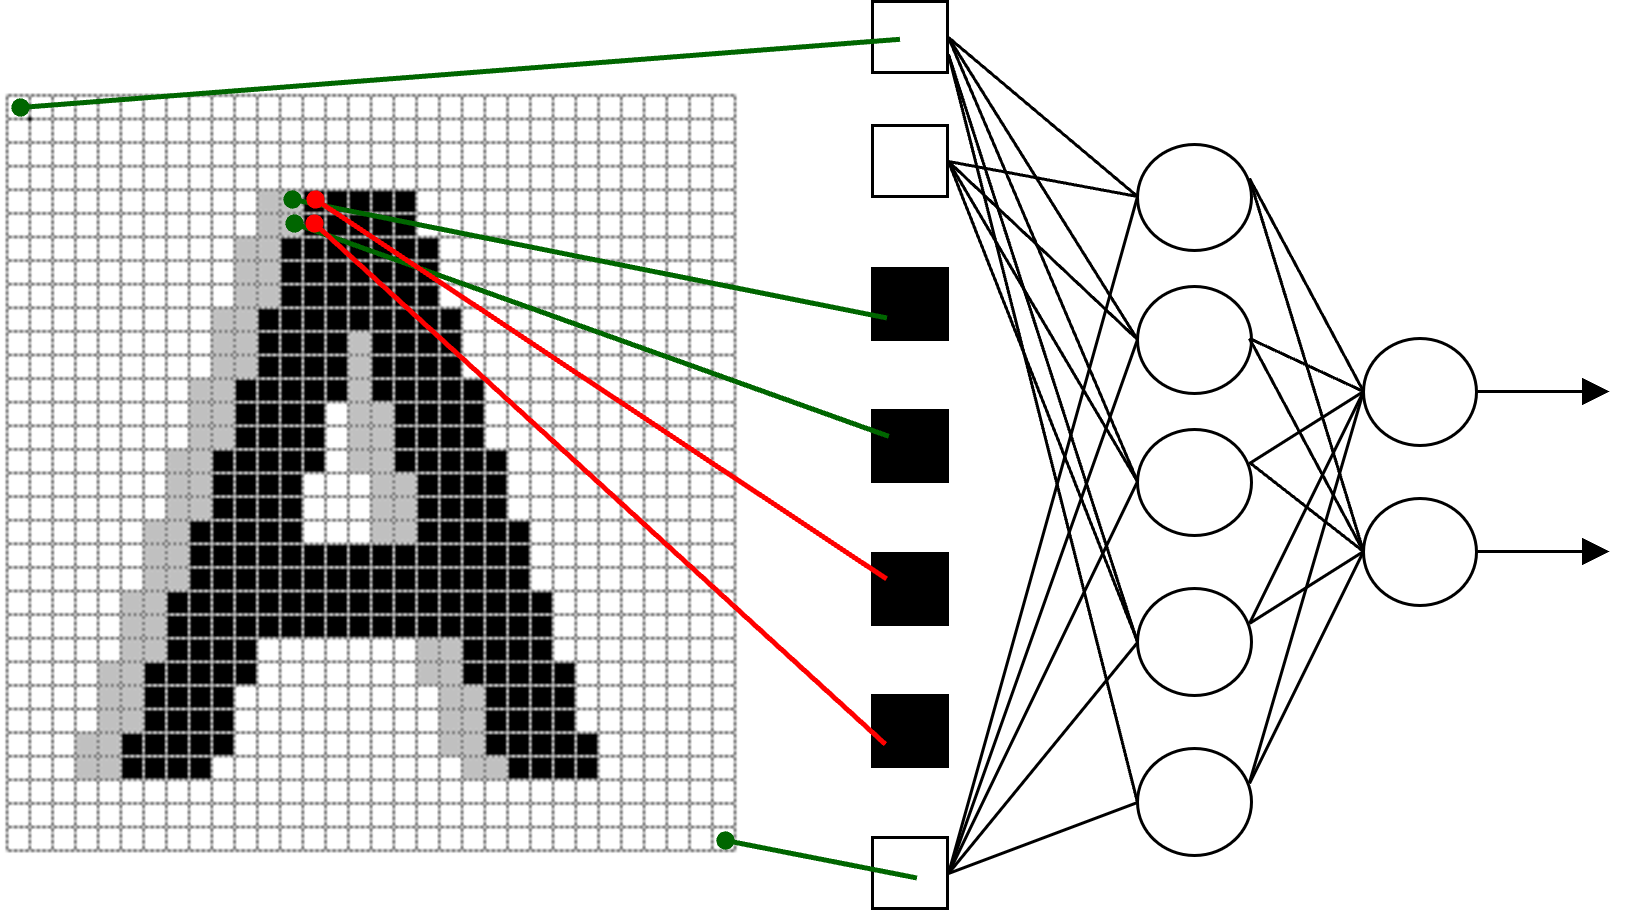
\includegraphics[width=\textwidth,height=0.7\textheight,keepaspectratio]{./images/nn_4.png}
    \caption{Shifted "A" character.}
    \label{fig:shifted_a}
\end{minipage}
\end{figure}


\framebreak

\begin{itemize}
    \item The topology of the input data is completely ignored (it treats pixels as independent features rather than structured patterns.)
    \item For a $32 \times 32$ image, we have
    \begin{itemize}
        \item Black and white patterns: $2^{32*32} = 2^{1024}$
        \item Grayscale patterns: $256^{32*32} = 256^{1024}$
    \end{itemize}
\end{itemize}

\begin{figure}
\centering

\includegraphics[width=1.0\textwidth,height=0.6\textheight,keepaspectratio]{./images/nn_5.png}
\end{figure}


\end{frame}

\framebreak

\begin{frame}{What do we need?}
\begin{itemize}
    \item We need a model that can:
    \begin{itemize}
        \item \textbf{Find Patterns in Images}: Recognize small features like edges and shapes in different parts of the image.
        \item \textbf{Work Efficiently}: Avoid looking at every pixel separately by focusing on groups of pixels together.
        \item \textbf{Handle Changes}: Still recognize the same object even if it moves, rotates, or looks slightly different.
    \end{itemize}
\end{itemize}


\end{frame}

\framebreak

\begin{frame}{What do we need?}
\begin{itemize}
    \item We need a model that can:
    \begin{itemize}
        \item \textbf{Find Patterns in Images}: Recognize small features like edges and shapes in different parts of the image.
        \item \textbf{Work Efficiently}: Avoid looking at every pixel separately by focusing on groups of pixels together.
        \item \textbf{Handle Changes}: Still recognize the same object even if it moves, rotates, or looks slightly different.
        \item We need \textbf{Convolutional Neural Networks (CNNs)!}

    \end{itemize}
\end{itemize}


\end{frame}

\framebreak

\begin{frame}{Convolutional Neural Networks (CNNs)}

\begin{itemize}
        \item CNNs are neural networks designed for image processing and consist of two main parts:

        \begin{itemize}
            \item \textbf{Feature Extractor}: Automatically learns patterns (features) such as edges, textures, and shapes from the image.
            \item \textbf{Classifier}: The extracted features are flattened into a vector and passed to a standard neural network (like the ones we used before) for classification.
    \end{itemize}
\end{itemize}

\begin{figure}
        \centering
        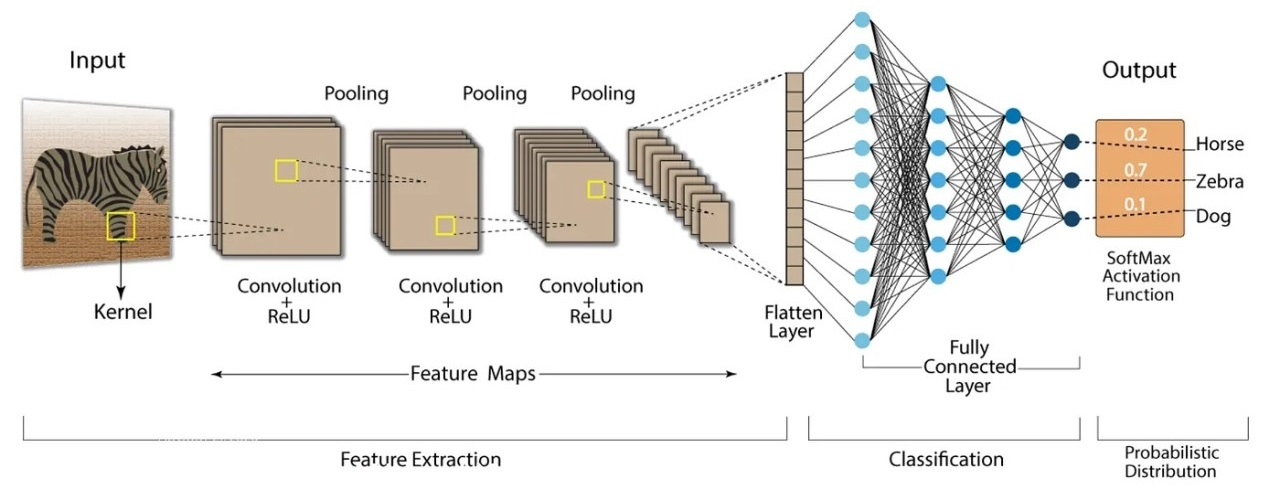
\includegraphics[width=0.9\textwidth,height=0.7\textheight,keepaspectratio]{./images/cnn_arch.jpeg}
        \caption{Convolutional Neural Network}

        \end{figure}
\end{frame}

\framebreak

\begin{frame}{Convolutional Neural Networks (CNNs)}
\begin{itemize}
    \item The feature extractor consists of three essential components:
    \begin{itemize}
        \item \textbf{Convolution Layers}: Detect local patterns such as edges, textures, and shapes by applying filters to the image.
        \item \textbf{Activation Function (ReLU)}: Adds non-linearity.
        \item \textbf{Pooling Layers}: Reduce the spatial size of extracted features.
    \end{itemize}
    \item Let's start with the convolution layer.
\end{itemize}

\end{frame}

\framebreak

\begin{frame}[allowframebreaks]{How Convolution Works?}

\begin{itemize}
    \item Let's consider this image.
\end{itemize}

\begin{figure}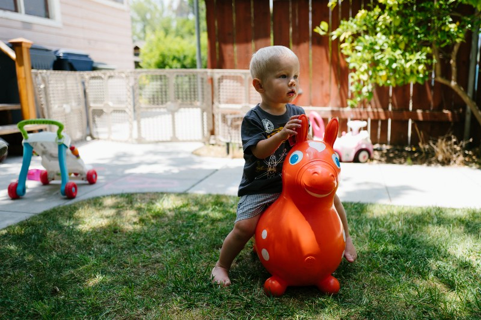
\includegraphics[width=0.8\textwidth,height=0.8\textheight,keepaspectratio]{./images/conv_2.png}
\end{figure}

\framebreak

\begin{enumerate}
    \item The image is divided into small overlapping tiles (regions).
\end{enumerate}

\begin{figure}
\centering
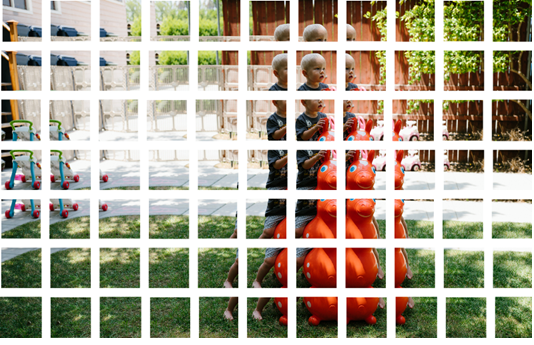
\includegraphics[width=0.8\textwidth,height=0.8\textheight,keepaspectratio]{./images/conv_3.png}
\end{figure}

\framebreak

\begin{enumerate}
    \setcounter{enumi}{1}
    \item We process each tile using the weights matrix of a small neural network. We call this matrix a \textbf{kernel} or \textbf{filter}.
\end{enumerate}

\begin{figure}
\centering
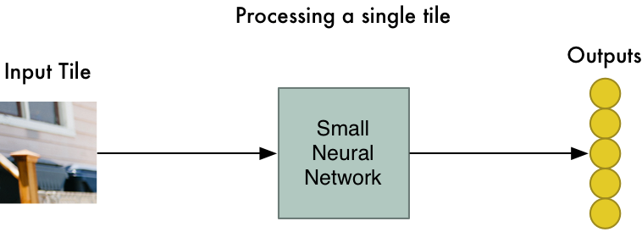
\includegraphics[width=1.0\textwidth,height=0.9\textheight,keepaspectratio]{./images/conv_4.png}
\end{figure}

\framebreak

\begin{enumerate}
    \setcounter{enumi}{2}
    \item Finally, the filter slides across the image (with the same weights) and processes all the tiles, creating an output \textbf{feature map}.
\end{enumerate}

\begin{figure}
\centering
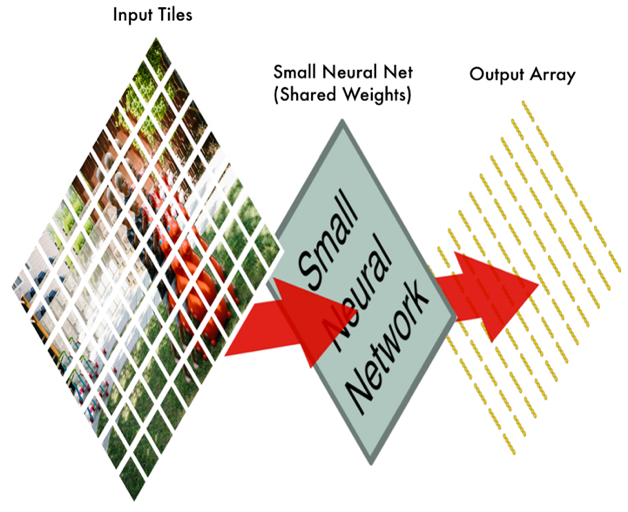
\includegraphics[width=0.8\textwidth,height=0.8\textheight,keepaspectratio]{./images/conv_5.png}
\end{figure}


\framebreak

\begin{itemize}
    \item What we did in the last step is called the \textbf{Convolution Operation}.
    \item We convolved the kernel with the image, which means sliding the kernel over the entire image and computing the dot product between the kernel and small regions of the image at each step.
    \begin{figure}
\centering
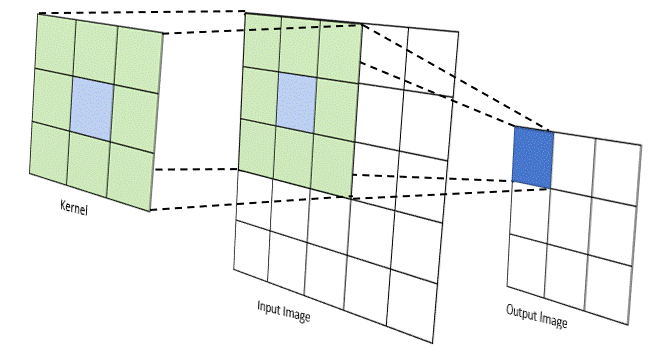
\includegraphics[width=0.8\textwidth,height=0.8\textheight,keepaspectratio]{./images/convolve.png}
\end{figure}

\end{itemize}



\framebreak

\begin{itemize}
    \item This can be represented mathematically by:
    
    \[
    z = W * x_{i,j} = \sum_{a=0}^{m-1} \sum_{b=0}^{n-1} W_{ab} X_{(i+a)(j+b)}
    \]
    \begin{itemize}
    \item $z$: Output of the convolution at $(i, j)$.
    \item $W$: Filter (kernel) matrix of size $m \times n$.
    \item $x_{i,j}$: Input value at position $(i, j)$.
    \item $W_{ab}$: Weight of the filter at $(a, b)$.
    \item $X_{(i+a)(j+b)}$: Input value in the small region at $(i+a, j+b)$.
    \end{itemize}

\end{itemize}



\framebreak

\begin{figure}
\centering
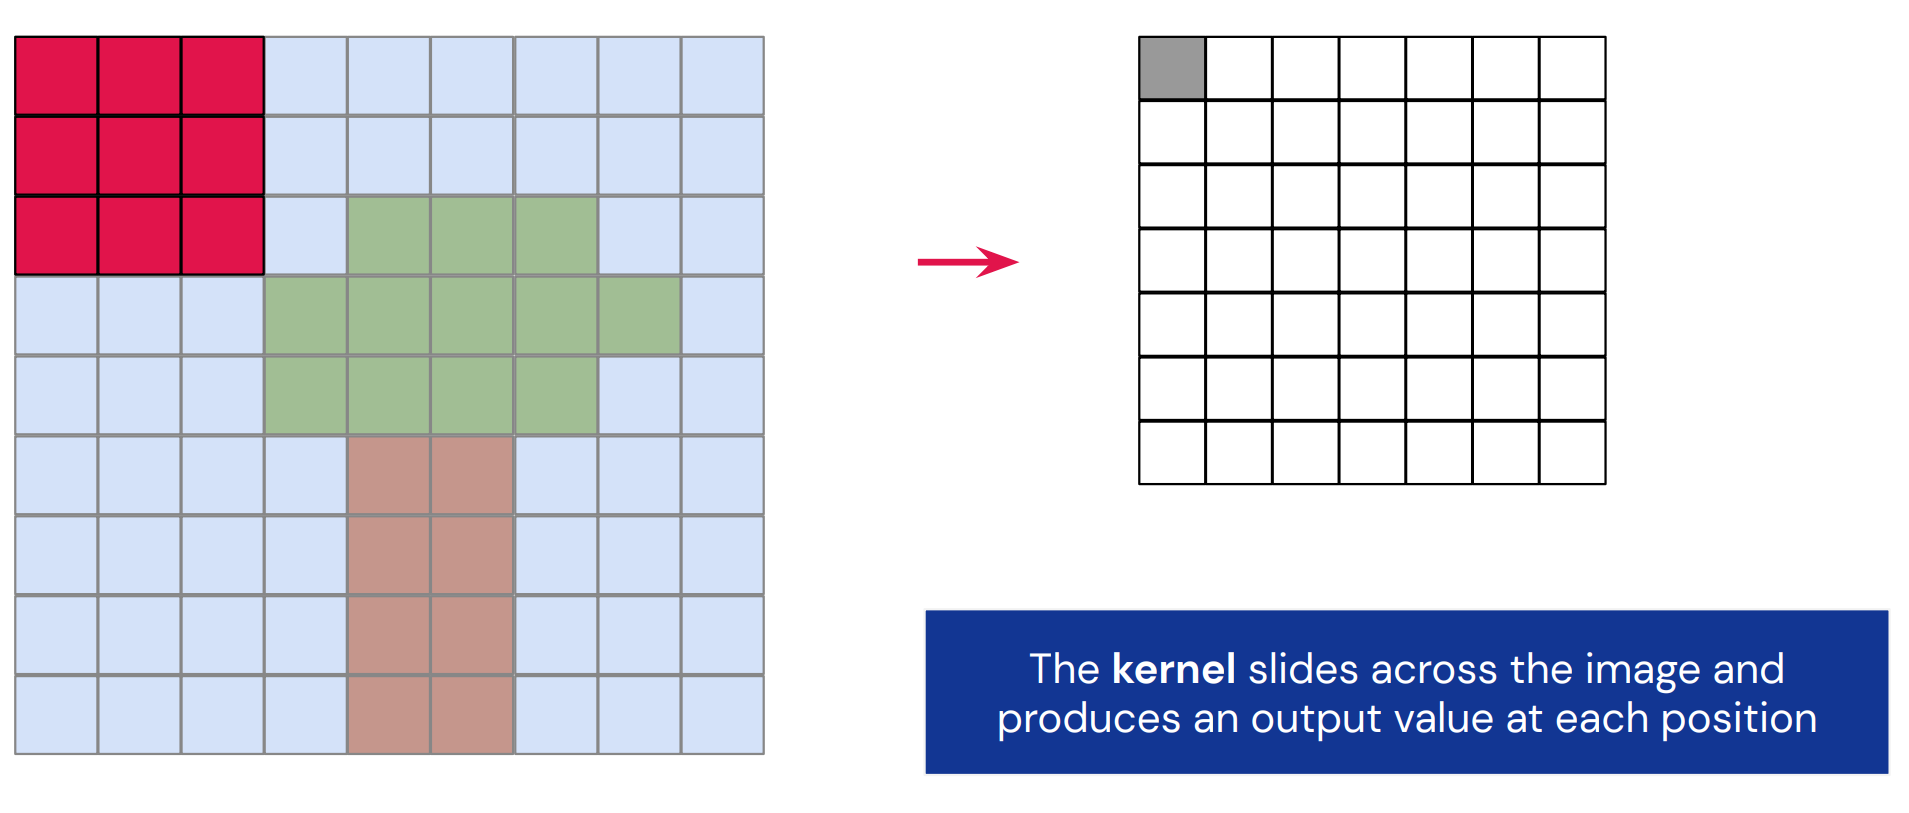
\includegraphics[width=1.0\textwidth,height=0.9\textheight,keepaspectratio]{./images/conv_7.png}
\end{figure}

\framebreak

\begin{figure}
\centering
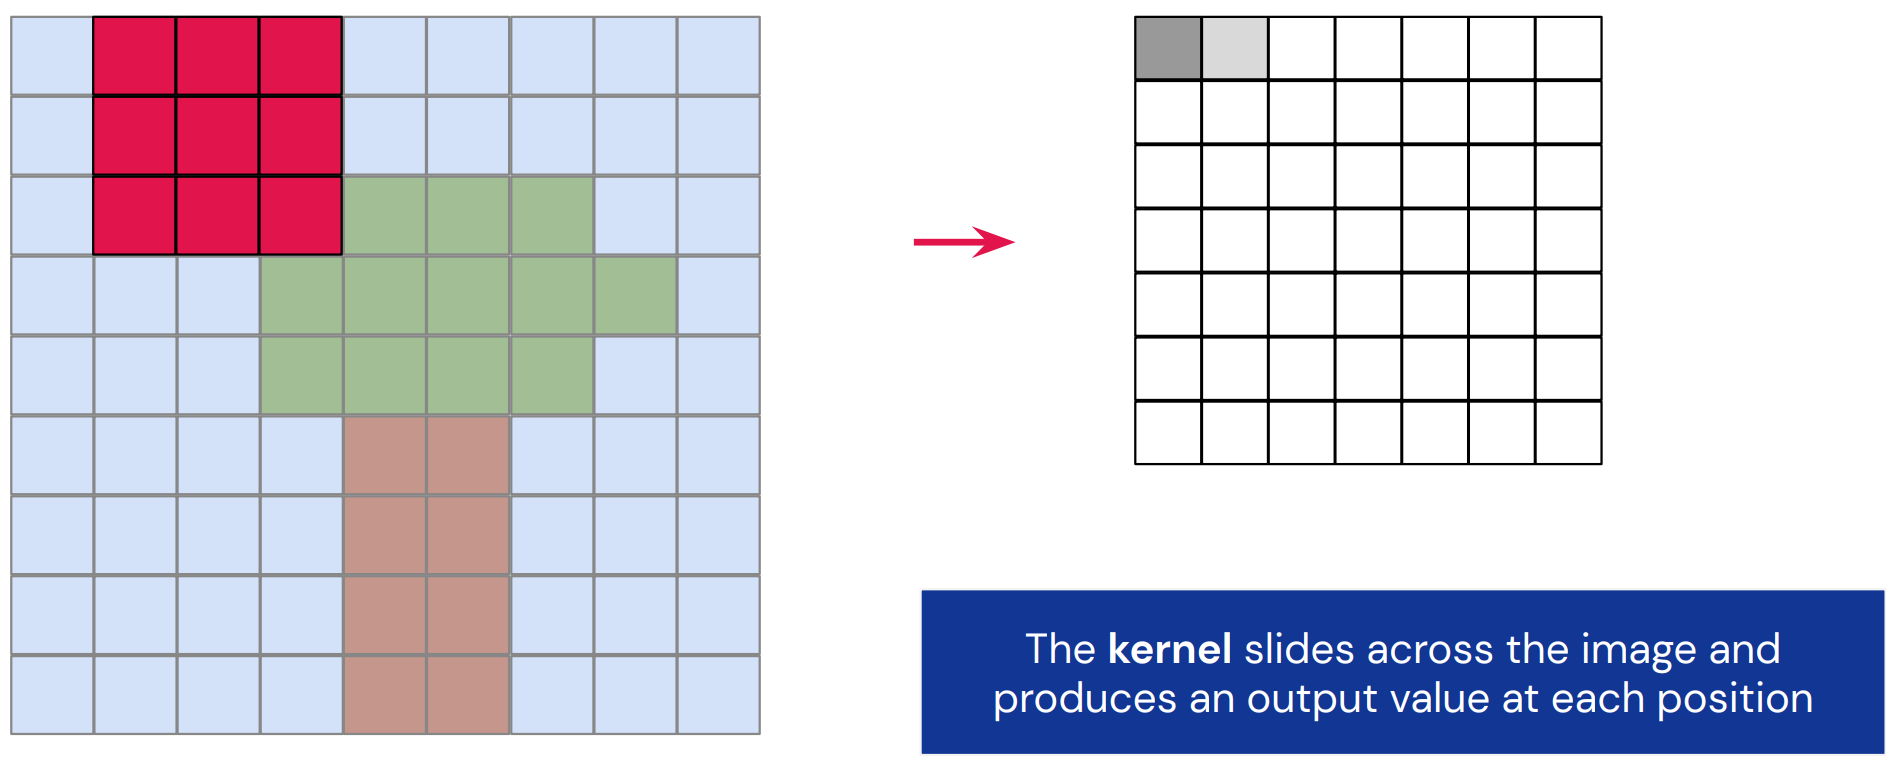
\includegraphics[width=1.0\textwidth,height=0.9\textheight,keepaspectratio]{./images/conv_8.png}
\end{figure}

\framebreak

\begin{figure}
\centering
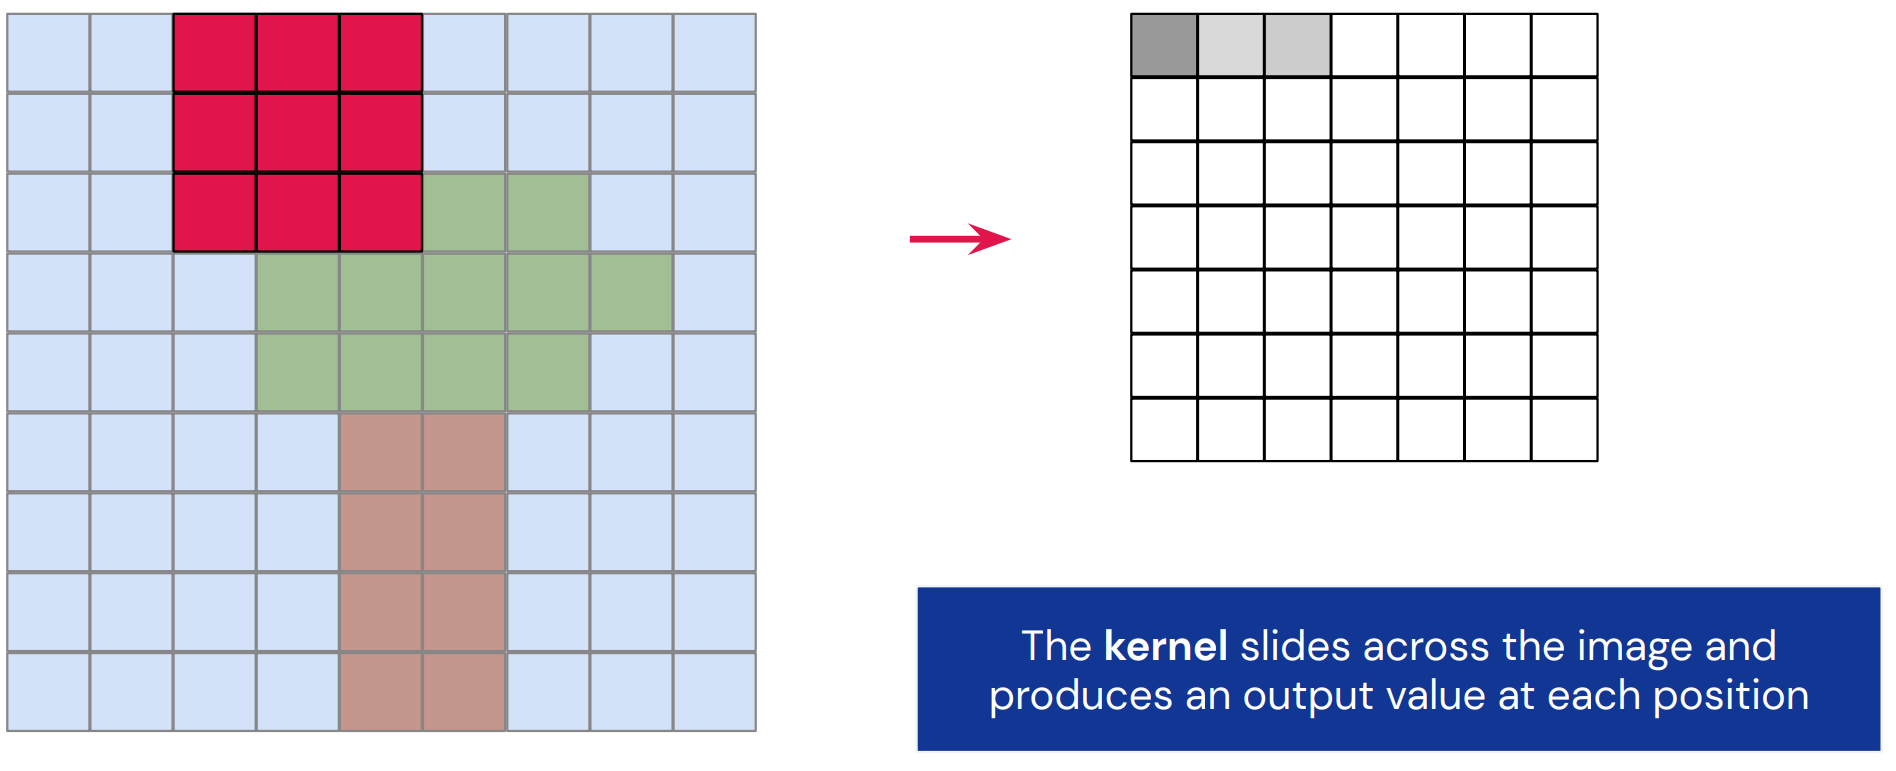
\includegraphics[width=1.0\textwidth,height=0.9\textheight,keepaspectratio]{./images/conv_9.png}
\end{figure}

\framebreak

\begin{itemize}
\item \textbf{Receptive Field}: The region of the input image that the kernel operates on at each step.
\item \textbf{Feature Map}: The features extracted from the input image.
\end{itemize}

\begin{figure}
\centering
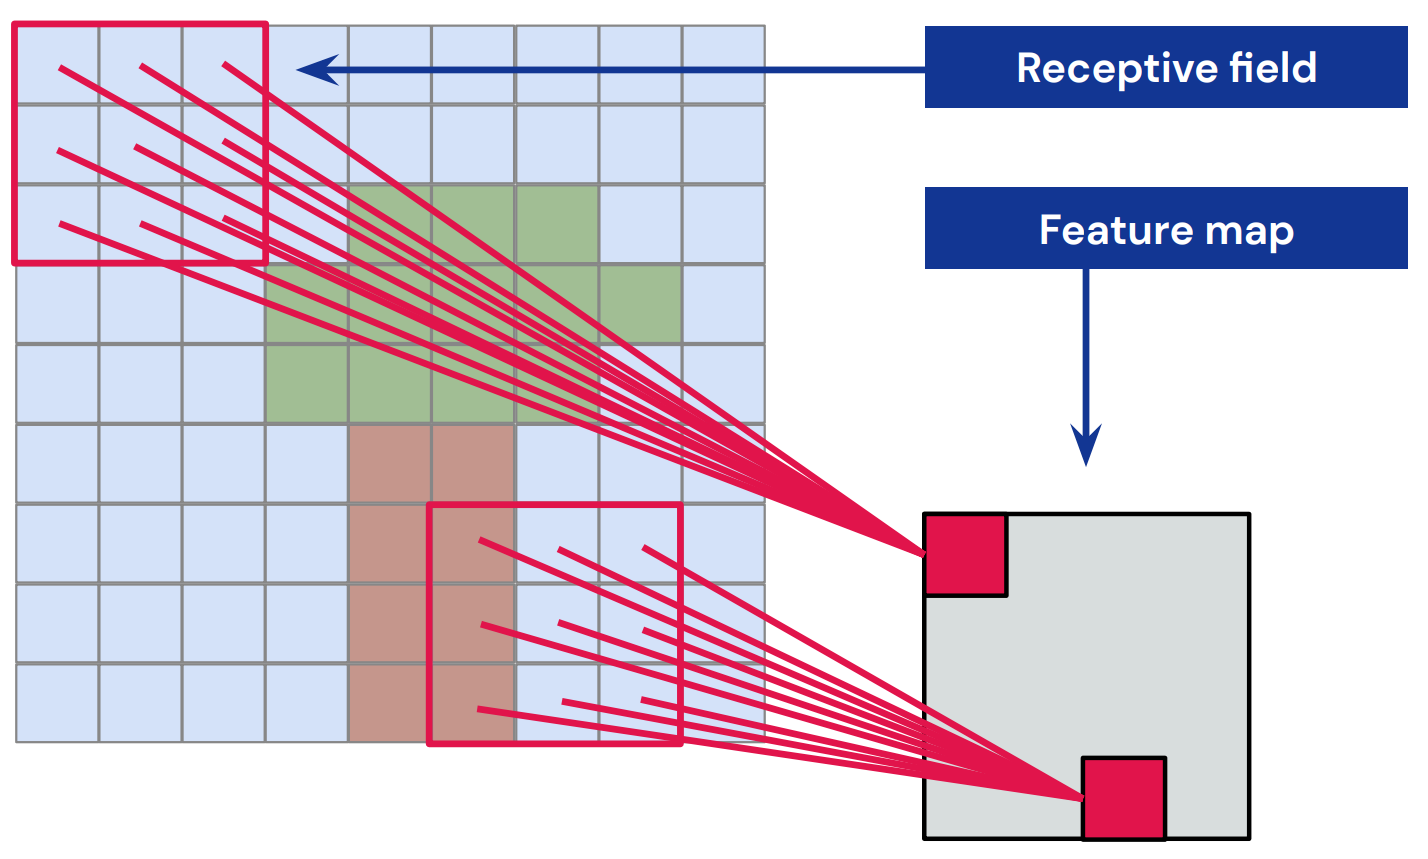
\includegraphics[width=0.8\textwidth,height=0.8\textheight,keepaspectratio]{./images/conv_10.png}
\end{figure}

\framebreak

\begin{figure}
\centering
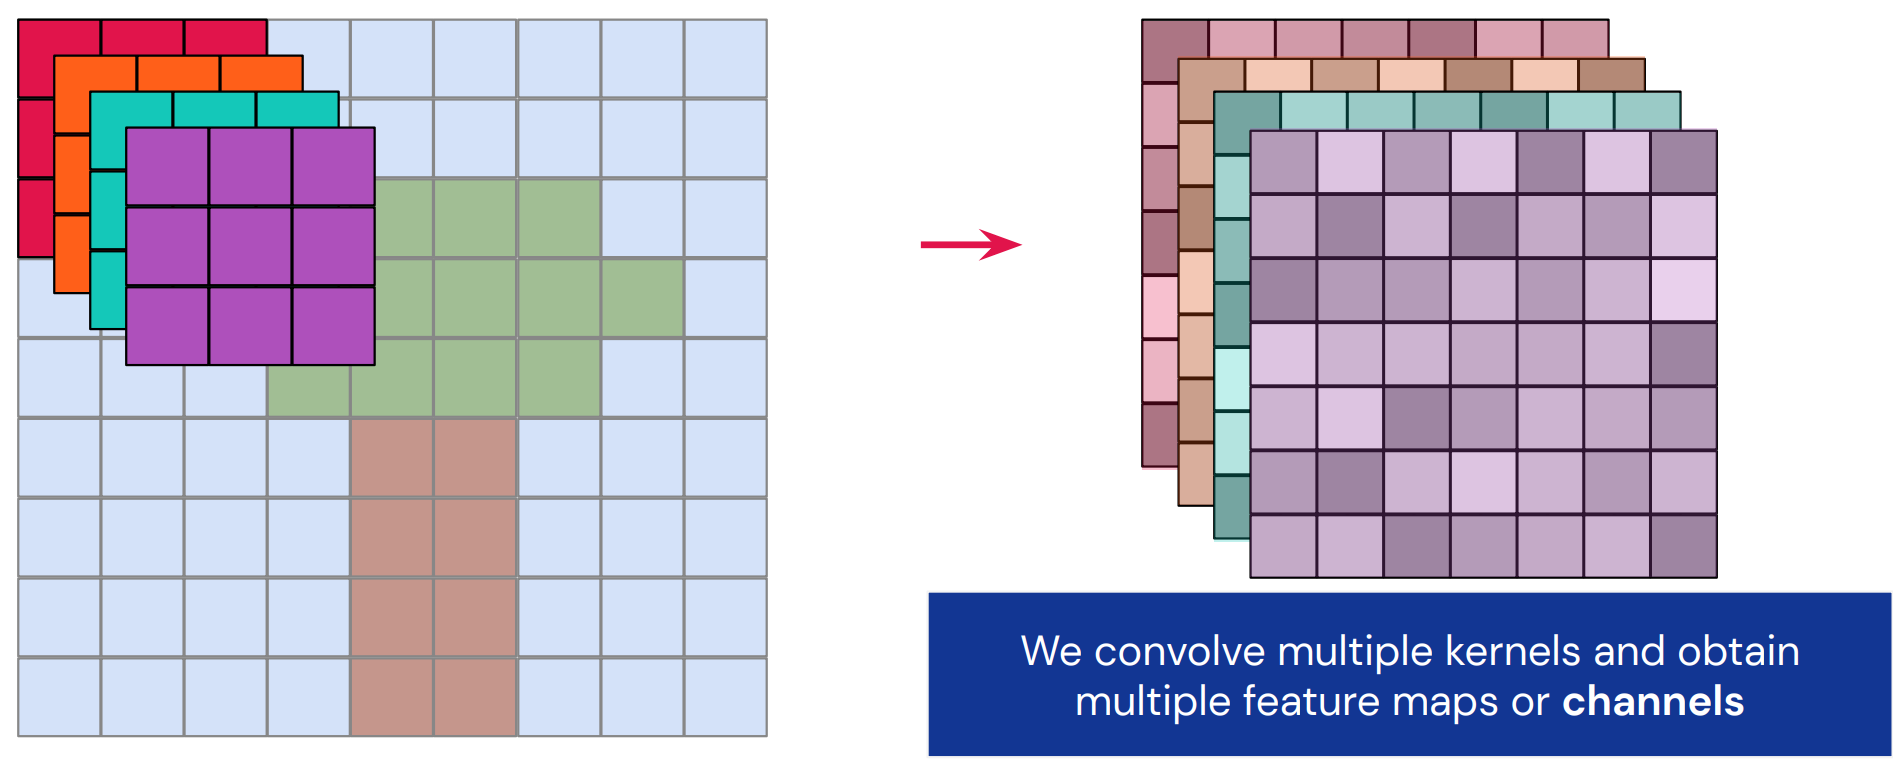
\includegraphics[width=1.0\textwidth,height=0.9\textheight,keepaspectratio]{./images/conv_11.png}
\end{figure}

\framebreak

\begin{itemize}
\item \textbf{Filters Example}: Different filters detect patterns like edges, textures, or smoothness, producing corresponding feature maps.
\end{itemize}

\begin{figure}
\centering
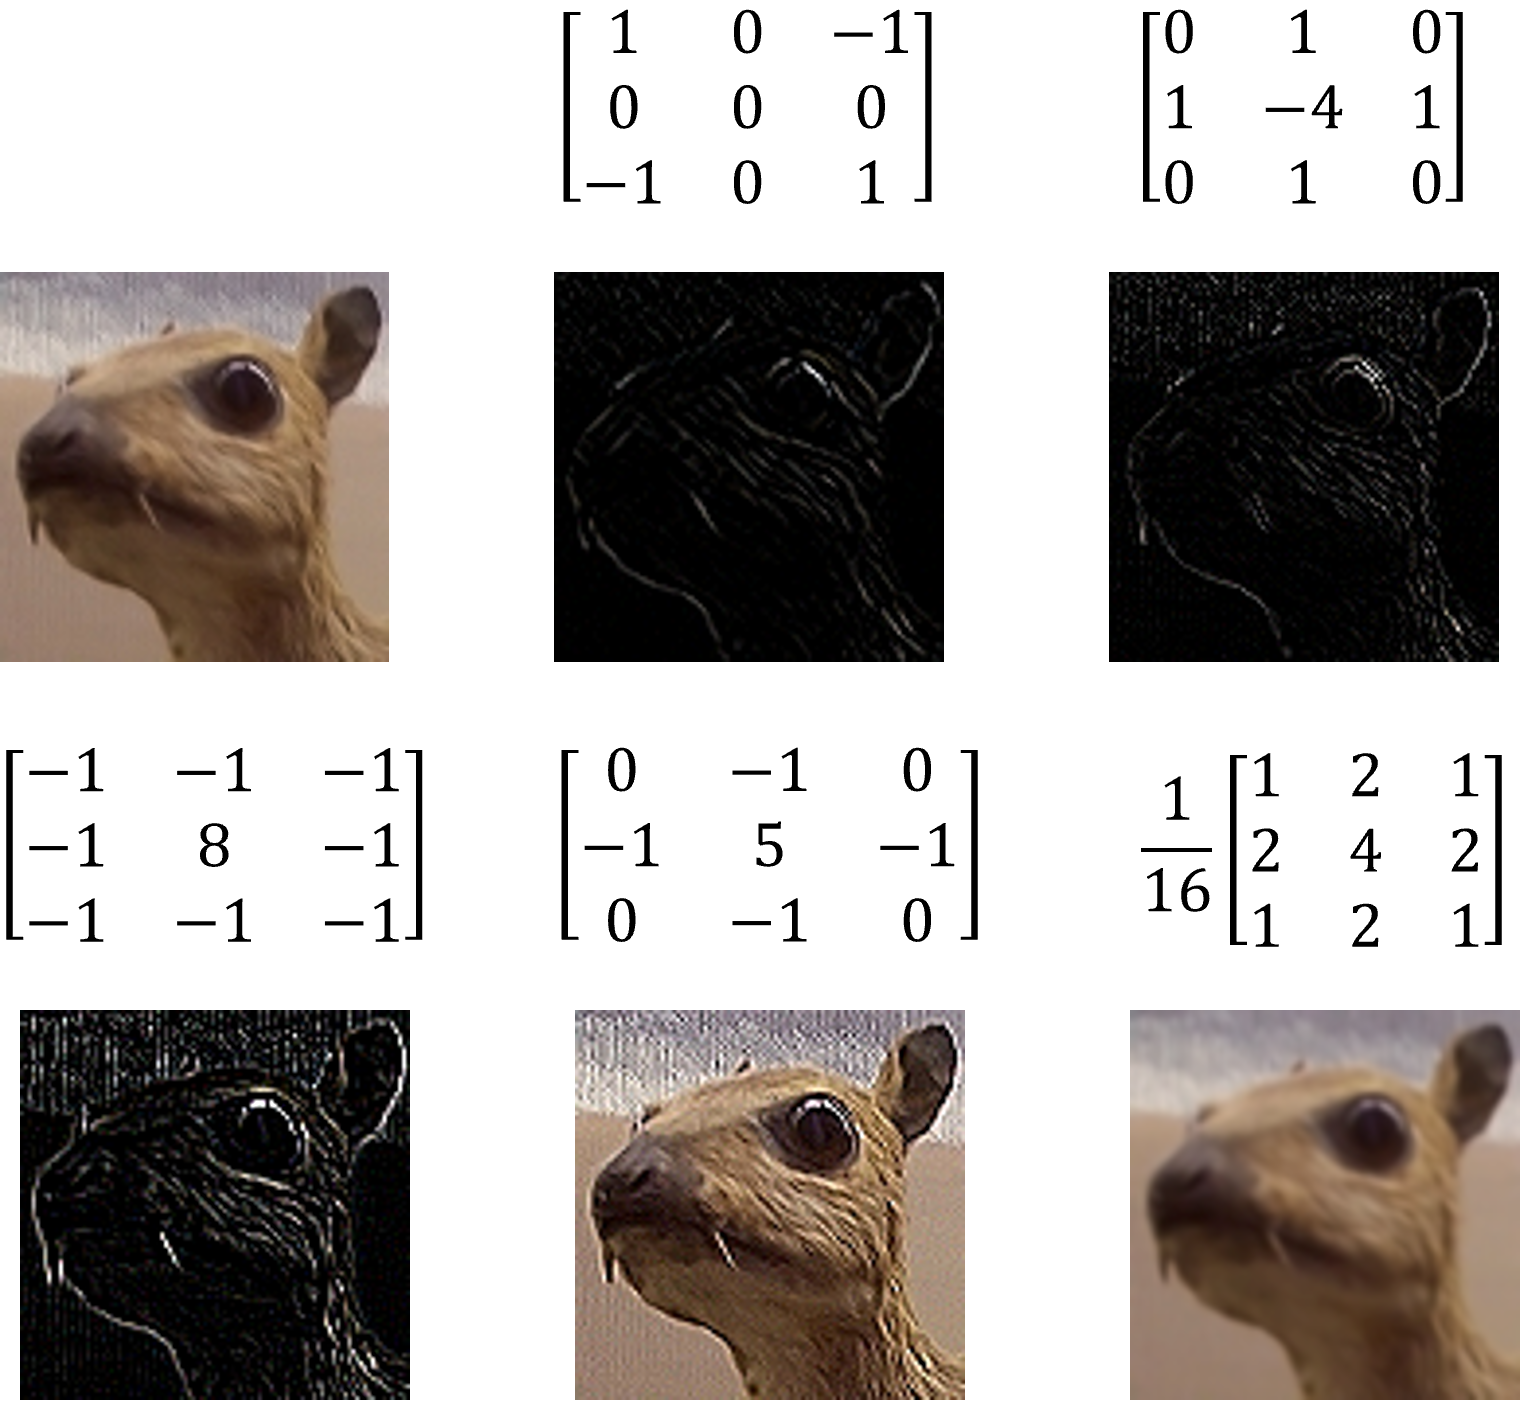
\includegraphics[width=0.8\textwidth,height=0.8\textheight,keepaspectratio]{./images/conv_12.png}
\end{figure}

    
\end{frame}


\begin{frame}[allowframebreaks]{Controlling the Convolution Process}
\begin{itemize}
    \item Applying Convolution as such reduces the size of the borders.
    \item Sometimes this is not desirable.
\end{itemize}


\begin{figure}
\centering
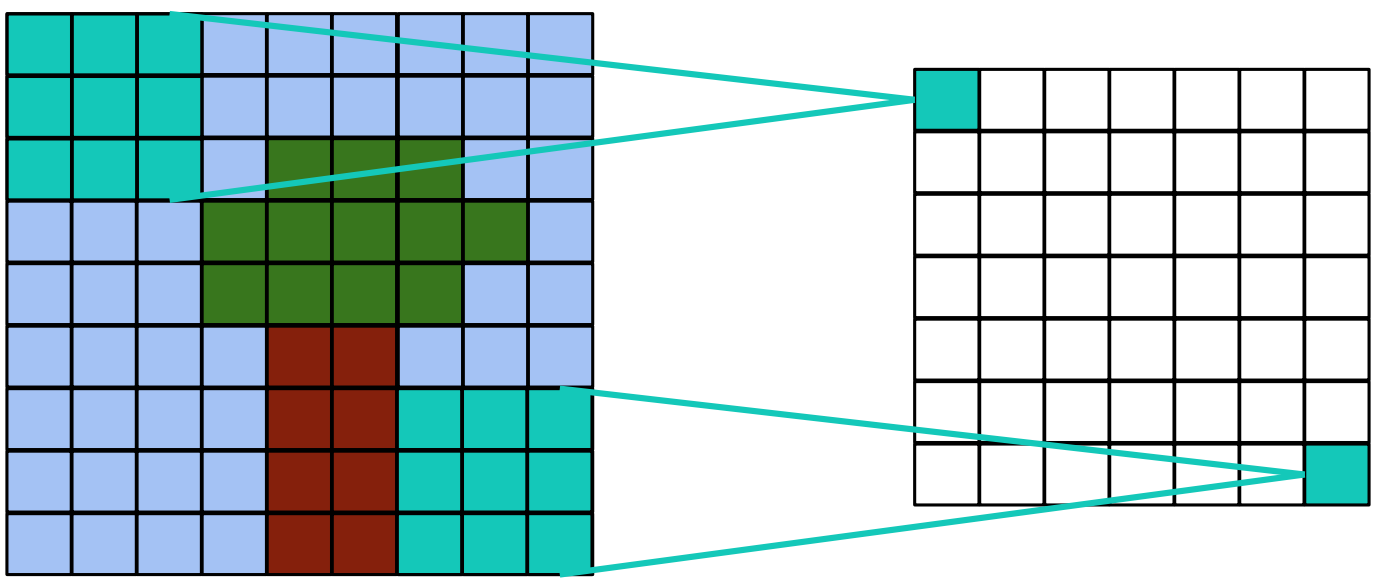
\includegraphics[width=1.0\textwidth,height=0.7\textheight,keepaspectratio]{./images/pad_1.png}
\end{figure}

\framebreak

\begin{itemize}
    \item Solution: We can use \textbf{Padding}, which pads the border with zeros.
    \item it has two types:
    \begin{enumerate}
    \item \textbf{Same Convolution}: Padding is added so the output size equals the input size.
    \end{enumerate}
\end{itemize}


\begin{figure}
\centering
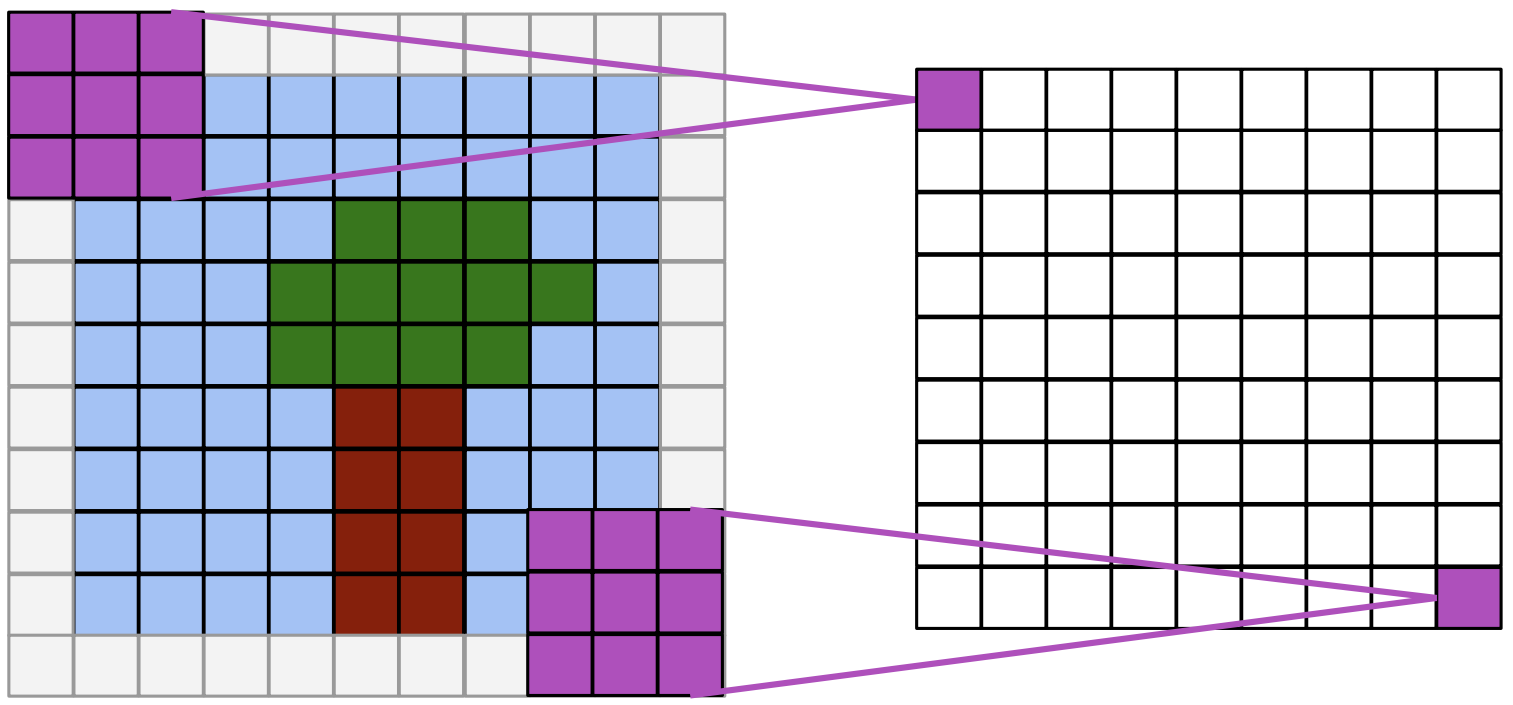
\includegraphics[width=1.0\textwidth,height=0.8\textheight,keepaspectratio]{./images/pad_3.png}
\end{figure}


\framebreak

\begin{itemize}
    \begin{enumerate}
    \setcounter{enumi}{1}
    \item \textbf{Full Convolution}:  Padding is added so the kernel covers the entire input, including edges. 
    \end{enumerate}
    \begin{itemize}
    output size = input size + kernel size - 1
    \end{itemize}
\end{itemize}


\begin{figure}
\centering
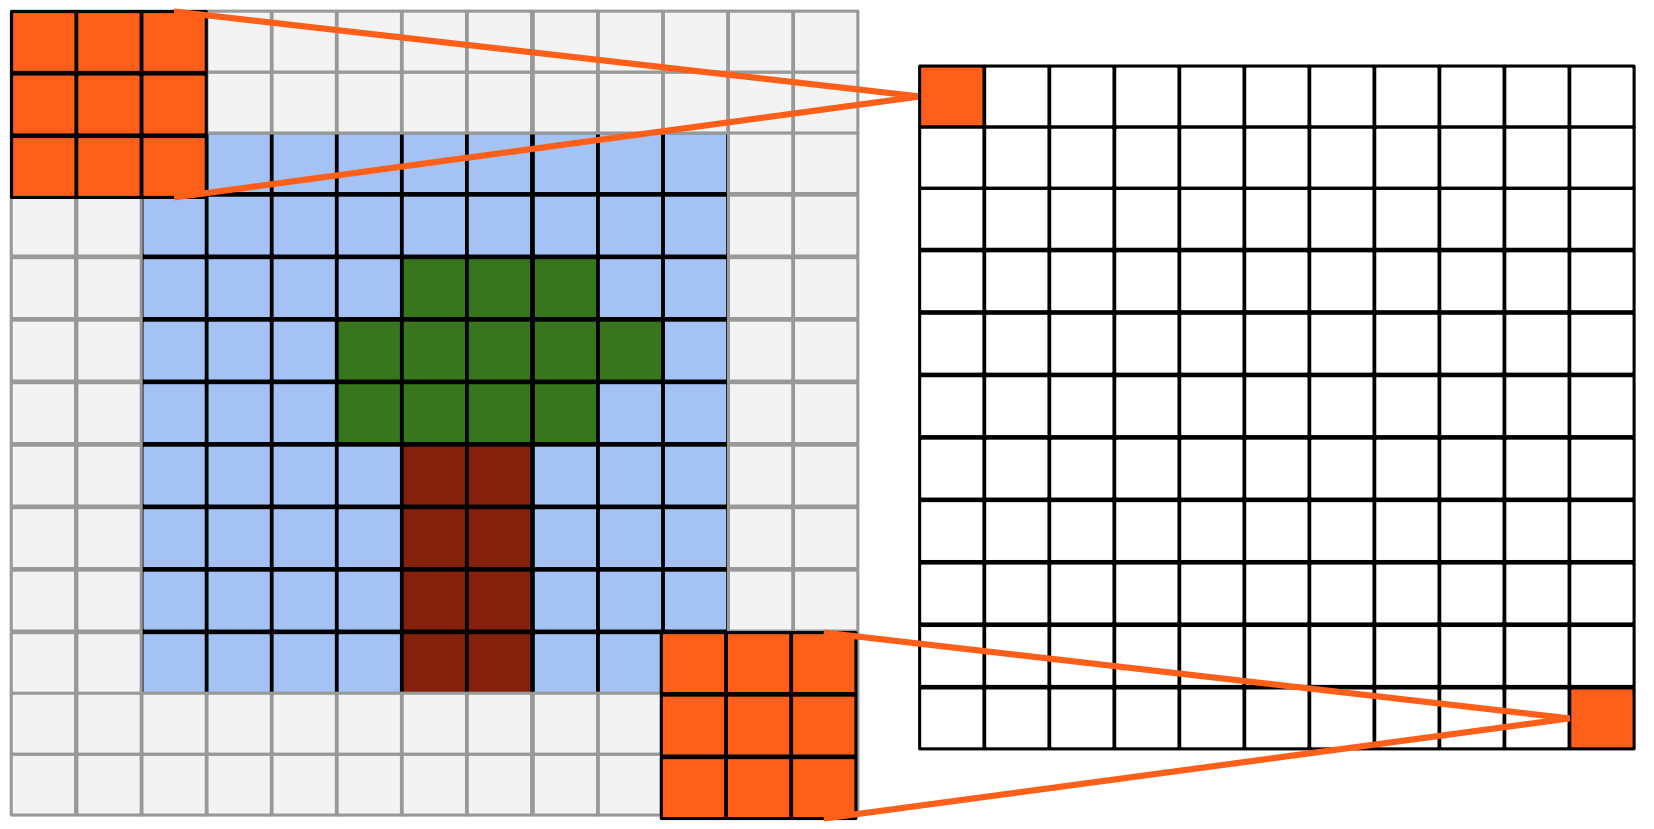
\includegraphics[width=1.0\textwidth,height=0.8\textheight,keepaspectratio]{./images/pad_2.png}
\end{figure}
    
\framebreak

\begin{itemize}
    \item \textbf{Strided Convolution}: Kernel slides along the image with a step $>$ 1
    \item Larger strides reduce output size.
\end{itemize}


\begin{figure}
\centering
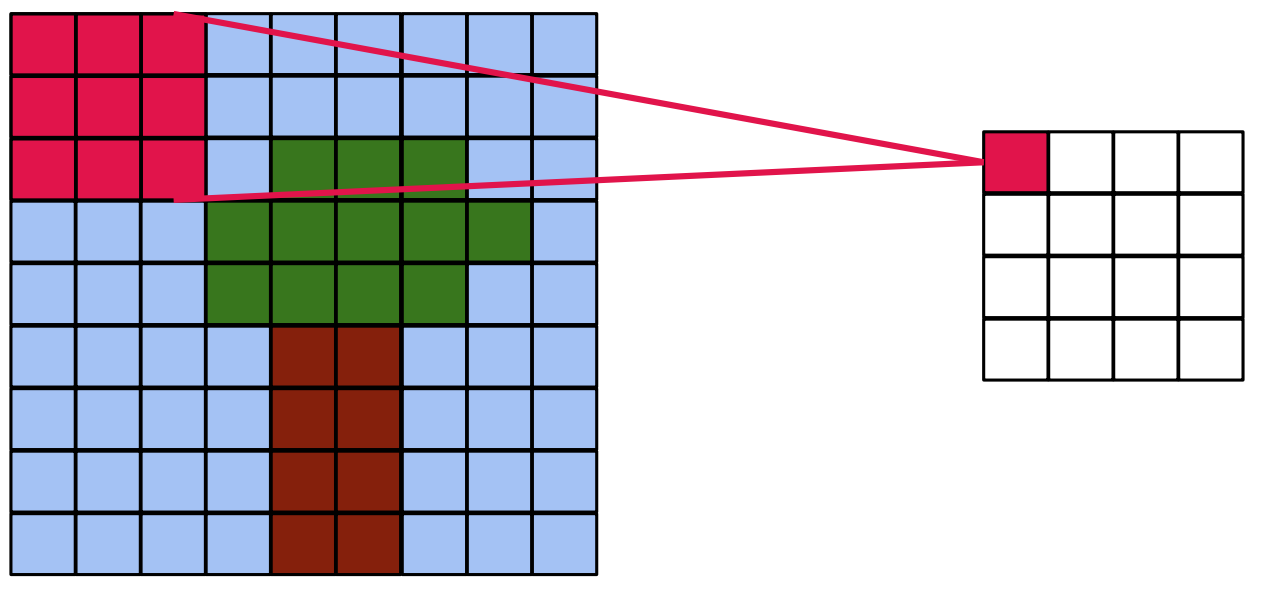
\includegraphics[width=1.0\textwidth,height=0.8\textheight,keepaspectratio]{./images/stride_1.png}
\end{figure}


\framebreak

\begin{itemize}
    \item \textbf{Strided Convolution}: Kernel slides along the image with a step $>$ 1
    \item Larger strides reduce output size.
\end{itemize}


\begin{figure}
\centering
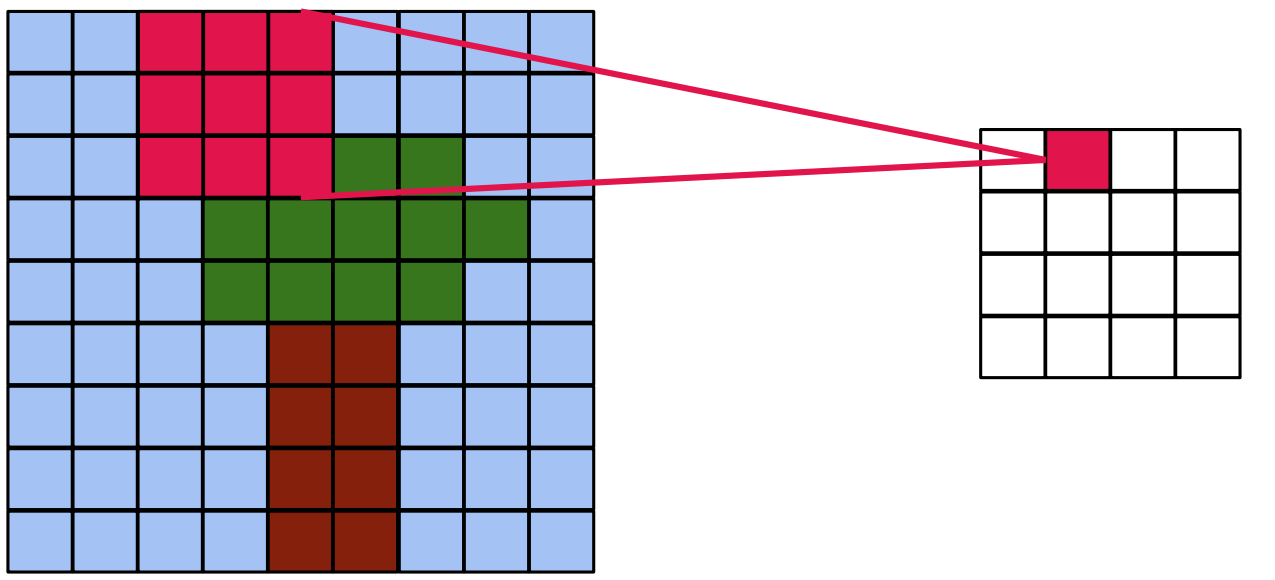
\includegraphics[width=1.0\textwidth,height=0.8\textheight,keepaspectratio]{./images/stride_2.png}
\end{figure}
    
\framebreak

\begin{itemize}
    \item \textbf{Pooling}: Compute mean or max over small windows to reduce resolution and extract more general features.
\end{itemize}


\begin{figure}
\centering
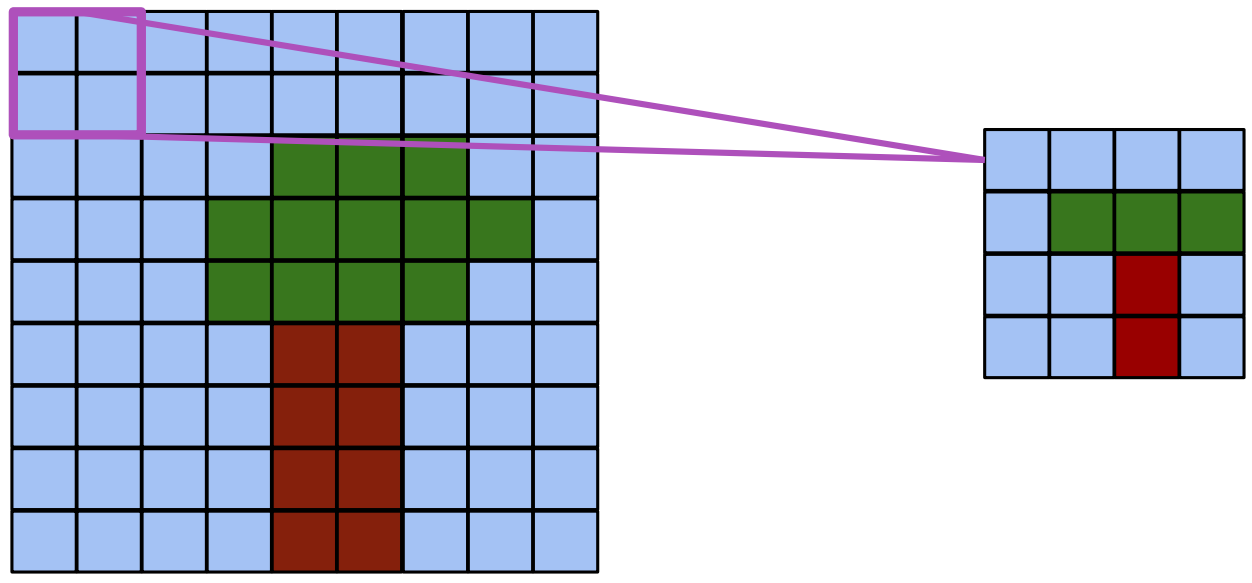
\includegraphics[width=1.0\textwidth,height=0.8\textheight,keepaspectratio]{./images/pool_1.png}
\end{figure}

\framebreak

\begin{figure}
\centering
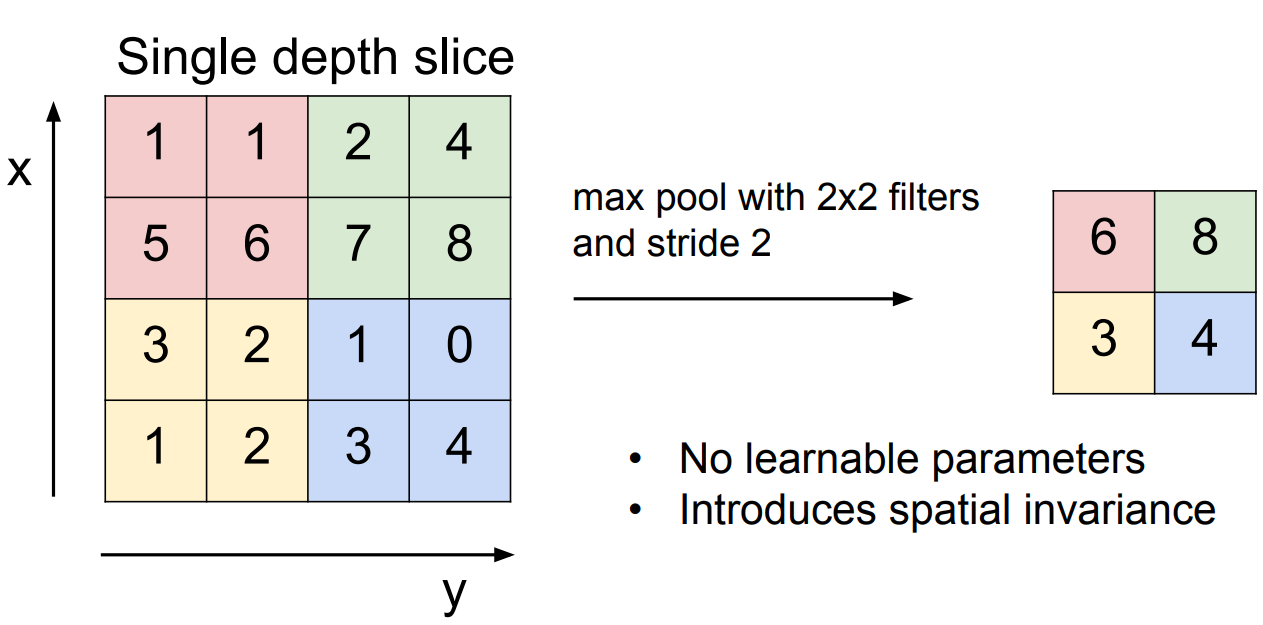
\includegraphics[width=1.0\textwidth,height=0.8\textheight,keepaspectratio]{./images/pool_2.png}
\end{figure}
    
\framebreak

\begin{itemize}
    \item \textbf{Dilated Convolution}: Kernel is spread out, step $>$ 1 between kernel elements.
    \item It expands the receptive field without increasing the number of parameters, which makes it efficient.
\end{itemize}


\begin{figure}
\centering
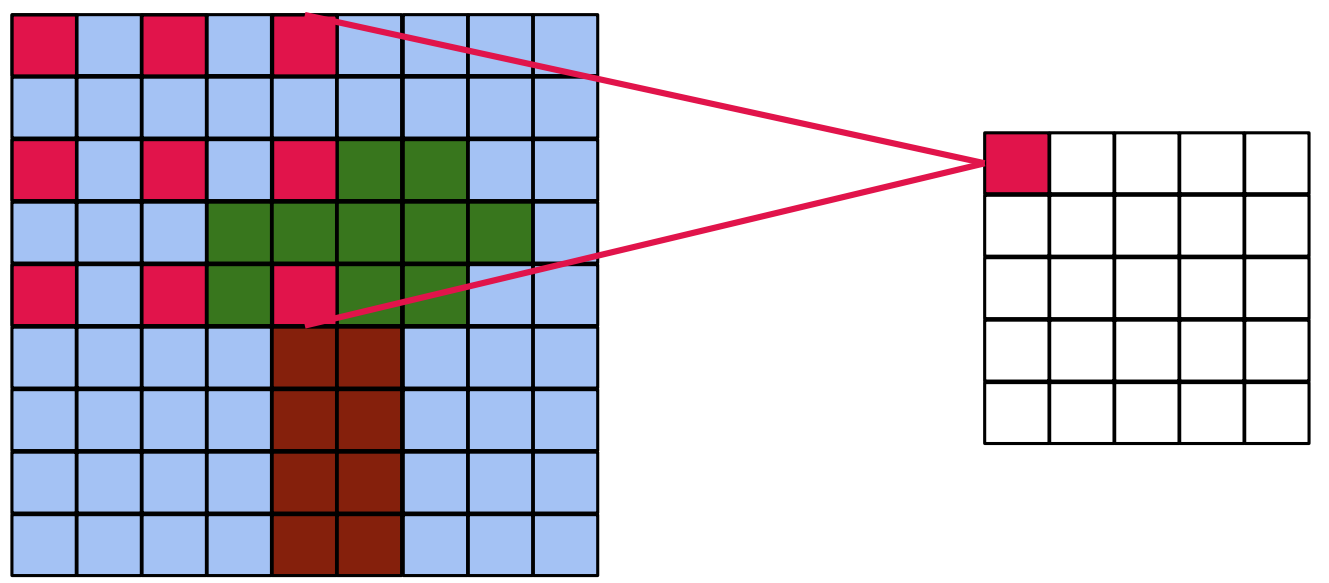
\includegraphics[width=1.0\textwidth,height=0.8\textheight,keepaspectratio]{./images/dilated.png}
\end{figure}

\end{frame}

\begin{frame}[allowframebreaks]{CNN Output size}


\[
n_{out} = \left\lfloor \frac{n_{in} + 2p - k}{s} \right\rfloor + 1
\]

\begin{align*}
n_{in} &: \text{number of input features} \\
n_{out} &: \text{number of output features} \\
k &: \text{convolution kernel size} \\
p &: \text{convolution padding size} \\
s &: \text{convolution stride size}
\end{align*}


\end{frame}

\begin{frame}{Activation}

\begin{itemize}
    \item Just like Fully-Connected Neural Networks, we can apply an activation over convolutional layer outputs
    \item It helps break linearity
    \item For example, Rectified Linear Unit (ReLU): $\sigma(x) = max(0,x)$
\end{itemize}


\begin{figure}
\centering
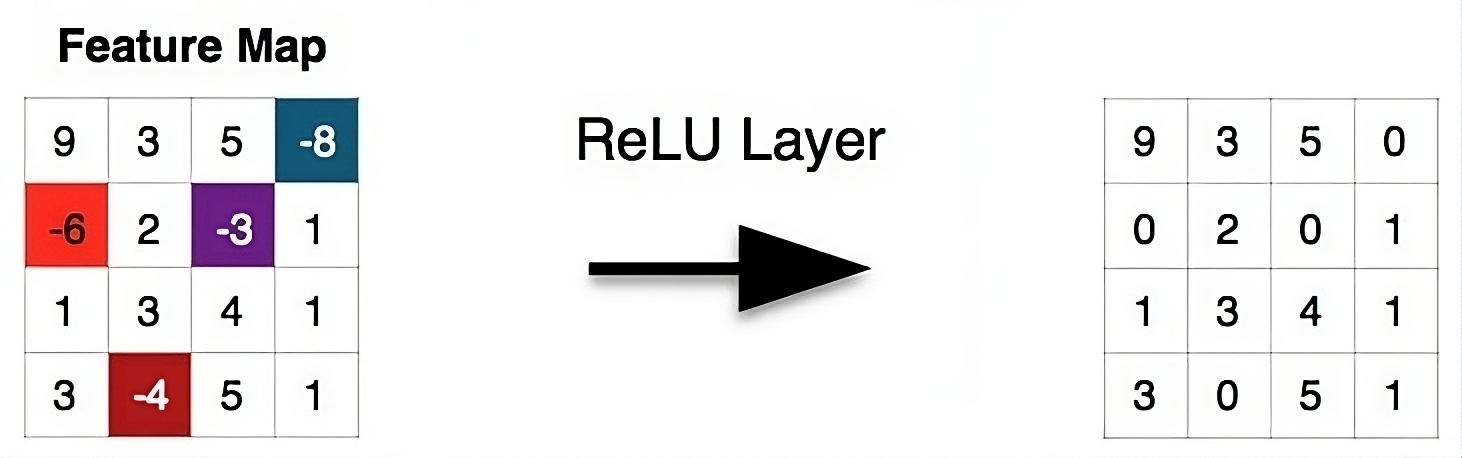
\includegraphics[width=1.0\textwidth,height=0.6\textheight,keepaspectratio]{./images/activation_relu.jpeg}
\end{figure}

\end{frame}



\begin{frame}{Convolutional Neural Networks}
\begin{figure}
\centering
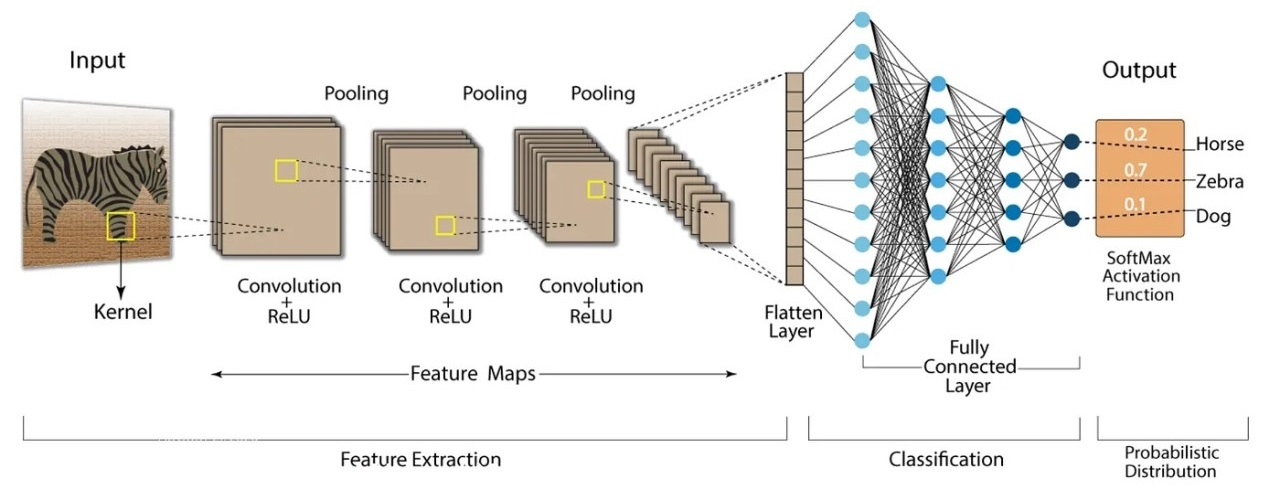
\includegraphics[width=1.0\textwidth,height=0.9\textheight,keepaspectratio]{./images/cnn_arch.jpeg}
\end{figure}
    
\end{frame}

\begin{frame}{Components of a CNN}
\begin{figure}
\centering
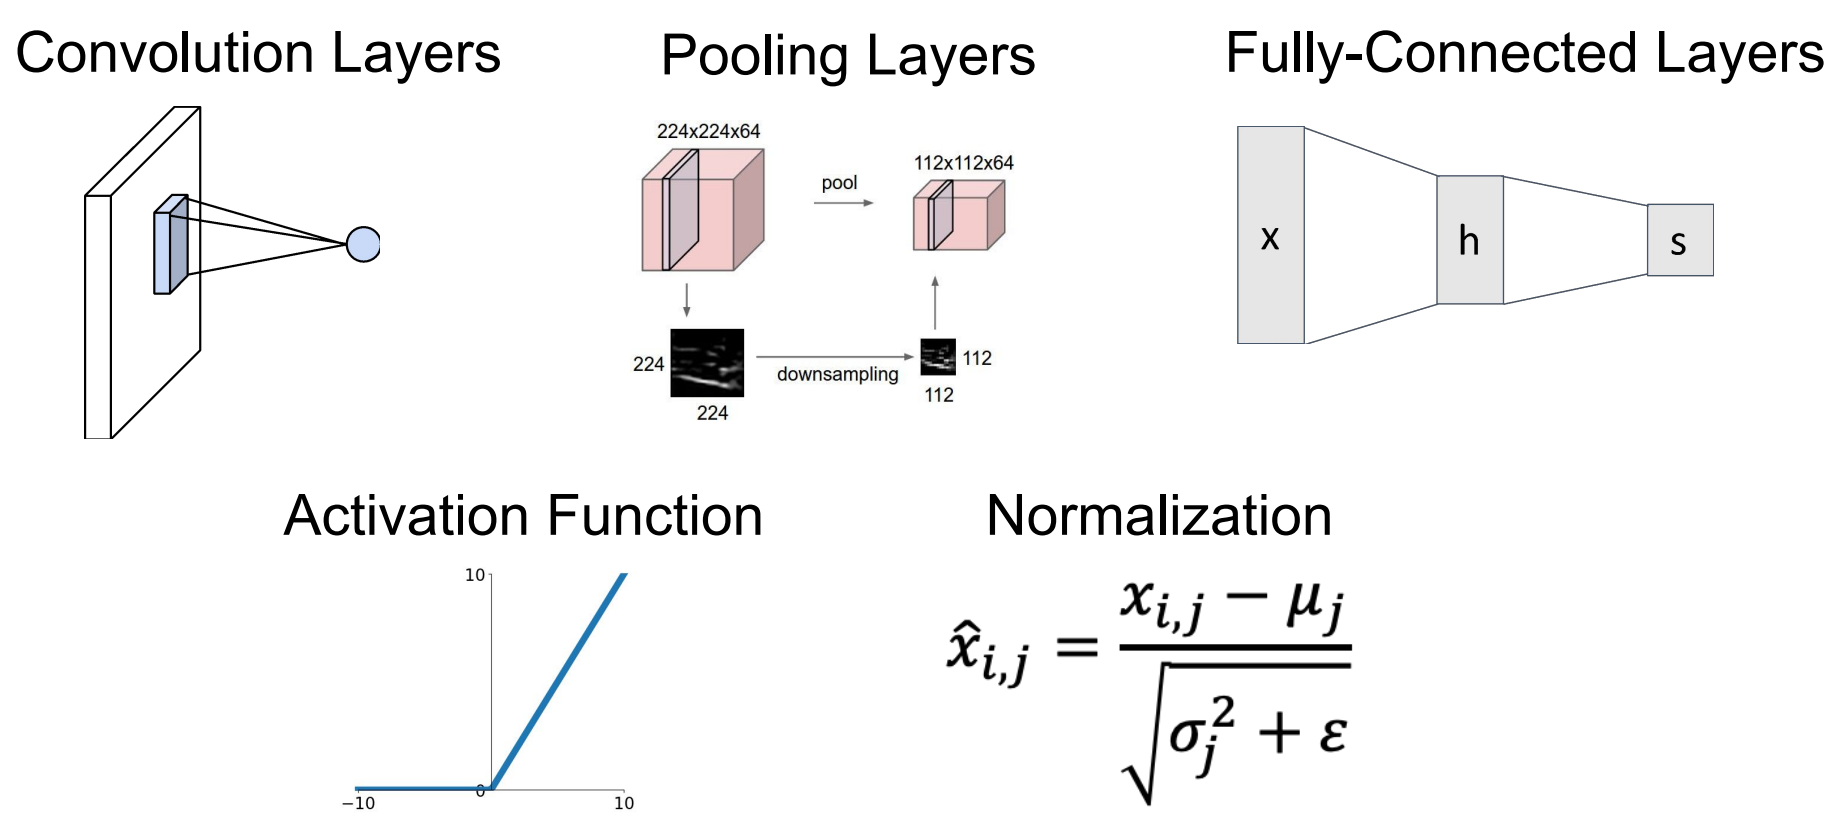
\includegraphics[width=1.0\textwidth,height=0.9\textheight,keepaspectratio]{./images/components.png}
\end{figure}
    
\end{frame}

\begin{frame}{Most Notable CNN-based Architectures}
\begin{itemize}
    \item Over time, researchers built advanced CNN architectures to improve performance and efficiency. These architectures introduced key innovations:
    \begin{itemize}
    \item \textbf{AlexNet \emph{[Krizhevsky et al. 2012]}}:  The first CNN to achieve breakthrough performance on image classification.
    \item \textbf{VGGNet \emph{[Simonyan and Zisserman, 2014]}}: Used very deep networks (up to 19 layers).
        \item \textbf{InceptionNet (GoogLeNet) \emph{[Szegedy et al., 2014]}}: Used multiple filter sizes per layer (Inception modules).
    \item \textbf{ResNet \emph{[He et al., 2015]}}: Introduced skip connections for training very deep networks.
    \item \textbf{EfficientNet \emph{[Tan and Le, 2019]}}: Found a scaling method that  simultaneously scales a CNN’s depth, width, and resolution optimally using a single scaling coefficient.
    \end{itemize}
    % \item DenseNet \emph{[Huang et al. 2017]}
\end{itemize}
    
\end{frame}

\begin{frame}{AlexNet}
\begin{itemize}
    \item First big improvement in image classification.
    \item Made use of CNN, pooling, dropout, ReLU and training on GPUs.
    \item 5 convolutional layers, followed by max-pooling layers; with three fully connected layers at the end

\end{itemize}

\begin{figure}
\centering
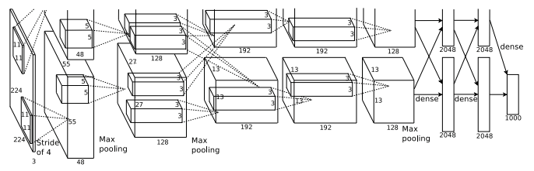
\includegraphics[width=1.0\textwidth,height=0.5\textheight,keepaspectratio]{./images/alexnet.png}
\end{figure}
    
\end{frame}

\begin{frame}{VGGNet}
\begin{itemize}
    \item \textbf{Improvement over AlexNet:} Uses a deeper network with small filters instead of a shallow network with larger filters.
    \item A stack of 3x3 conv layers (vs. 11x11 conv) has same receptive field, more non-linearities, fewer parameters and deeper network representation.
    \item Two variants: VGG16 or VGG19 conv layers plus 3 FC layers.
\end{itemize}

\begin{figure}
\centering
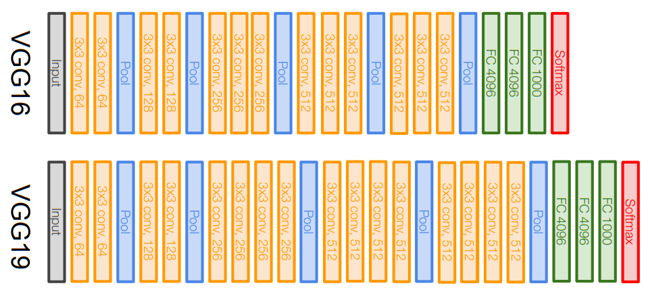
\includegraphics[width=1.0\textwidth,height=0.5\textheight,keepaspectratio]{./images/VGG_16_19.png}
\end{figure}
    
\end{frame}

\begin{frame}[allowframebreaks]{InceptionNet}
    \begin{itemize}
        \item Going Deep: 22 layers
        \item Only 5 million parameters! (12× fewer than AlexNet, 27× fewer than VGGNet).
        \item Introduced efficient "Inception module"
        \item Introduced "bottleneck" layers that use 1x1 convolutions to reduce the number of channels and mix information across them.
    \end{itemize}

\begin{figure}
\centering
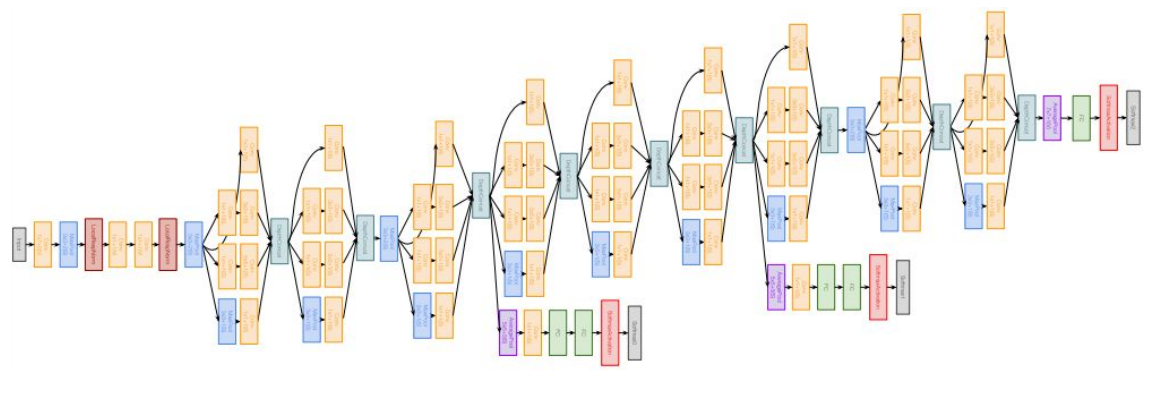
\includegraphics[width=1.0\textwidth,height=0.5\textheight,keepaspectratio]{./images/inceptionnet_1.png}
\end{figure}

\framebreak

    \begin{itemize}
        \item \textbf{Inception module:} Uses multiple filter sizes (1×1, 3×3, 5×5), in parallel, to capture different features, then combines their outputs.

    \end{itemize}

\begin{figure}
\centering
\includegraphics[width=1.0\textwidth,height=0.8\textheight,keepaspectratio]{./images/inception_mod.png}
\end{figure}

\end{frame}

\begin{frame}{ResNet: Motivation}
    \begin{itemize}
        \item \textbf{Problem:} Making networks deeper does not always improve accuracy.
        \item \textbf{Why?} In very deep networks, gradients become extremely small as they move backward through layers, making learning slow or stopping it altogether (\textbf{vanishing gradient problem}).
        \item \textbf{Solution:} Residual Network (ResNet) introduces \textbf{skip connections (residuals)}, allowing information to flow more easily.

    \end{itemize}
\end{frame}



\begin{frame}{ResNet}
\begin{itemize}
    \item Very deep networks using residual connections
    \item 152-layer model for ImageNet
    \item Stacked Residual Blocks
    \item \textbf{Residual:} A shortcut connection that helps the network pass information through layers more easily.


\end{itemize}

\begin{figure}
\centering
\includegraphics[width=1.0\textwidth,height=0.6\textheight,keepaspectratio]{./images/resnet_1.png}
\end{figure}
    
\end{frame}

\begin{frame}{ResNet}
\begin{itemize}
    \item What happens when we continue stacking deeper layers on a "plain" convolutional 
neural network?

\end{itemize}
\pause
\begin{figure}
\centering
\includegraphics[width=1.0\textwidth,height=0.5\textheight,keepaspectratio]{./images/resnet_2.png}
\end{figure}

\pause
\begin{itemize}
    \item 56-layer model performs worse on both test and training error
    \pause
    \item The deeper model performs worse, but it’s not caused by overfitting!
\end{itemize}

\end{frame}


\begin{frame}{ResNet}
\begin{itemize}
    \item \textbf{Fact:} Deep models have more representation power (more parameters) than shallower models.
    \pause
    \item \textbf{Hypothesis:} The problem is an optimization problem, deeper models are harder to optimize
    \pause
    \item \textbf{Solution:} Use network layers to fit a residual mapping instead of directly trying to fit a 
 desired underlying mapping

\end{itemize}
\pause
\begin{figure}
\centering
\includegraphics[width=1.0\textwidth,height=0.5\textheight,keepaspectratio]{./images/resnet_3.png}
\end{figure}


\end{frame}

\begin{frame}{ImageNet}
\begin{itemize}
    \item The most extensive data for Image Classification
    \item 3 RGB channels from 0 to 255
    \item 14,197,122 images
    \item 1000 classes
\end{itemize}

\begin{figure}
\centering
\includegraphics[width=1.0\textwidth,height=0.5\textheight,keepaspectratio]{./images/imagenet.png}
\end{figure}
\end{frame}

\begin{frame}{ImageNet Large Scale Visual Recognition Challenge (ILSVRC) winners}
\begin{figure}
\centering
\includegraphics[width=1.0\textwidth,height=1.0\textheight,keepaspectratio]{./images/imagenet_2.png}
\end{figure}

    
\end{frame}

\begin{frame}{EfficientNet: Motivation}
\begin{itemize}
    \item \textbf{Problem:} To improve accuracy, we can:
    \begin{itemize}
        \item Increase the number of layers (\textbf{depth})
        \item Increase the number of neurons in each layer (\textbf{width})
        \item Use higher-resolution images (\textbf{resolution})
    \end{itemize}
    But finding the right balance of these three was largely based on trial and error.
    
    \item \textbf{Solution:} EfficientNet introduced a \textbf{compound scaling} method—a mathematical formula to systematically find the optimal balance among \textbf{depth}, \textbf{width}, and \textbf{resolution}.
\end{itemize}
\end{frame}

\begin{frame}{EfficientNet}

    \begin{figure}
        \centering
        % Replace with your own figure path
        \includegraphics[width=\linewidth]{./images/ENet_1.png}
        \caption{EfficientNet Scaling.}
    \end{figure}
\end{frame}


\begin{frame}{EfficientNet}
    \begin{itemize}
        \item \textbf{Compound Scaling} Uses a single \textbf{scaling coefficient} (\(\phi\)) to control:
        \begin{itemize}
        \item \textbf{Network Depth} (\(\alpha^\phi\)) → More layers
        \item \textbf{Network Width} (\(\beta^\phi\)) → More channels per layer
        \item \textbf{Input Resolution} (\(\gamma^\phi\)) → Larger input images
    \end{itemize}
        \item The goal: find \(\alpha, \beta, \gamma\) that balance accuracy \& efficiency, then scale up optimally by increasing the global coefficient \(\phi\).
    \end{itemize}

\end{frame}

\begin{frame}{EfficientNet}
\begin{itemize}
    \item EfficientNet optimizes depth, width, and resolution using this constraint:
    \[
    \alpha \cdot \beta^2 \cdot \gamma^2 \approx 2
    \]
    \item \textbf{Why this equation?}
    \begin{itemize}
        \item Increasing \textbf{depth} (\(\alpha\)) increases FLOPs \textbf{linearly}.
        \item Increasing \textbf{width} (\(\beta\)) increases FLOPs \textbf{quadratically} (\(\beta^2\)).
        \item Increasing \textbf{resolution} (\(\gamma\)) increases FLOPs \textbf{quadratically} (\(\gamma^2\)).
    \end{itemize}
    \item To double total FLOPs, the three factors must be balanced together.
\end{itemize}
\end{frame}



\begin{frame}{EfficientNet}
\begin{itemize}
    \item The authors of EfficientNet searched for the best scaling factors on a small baseline model.
    \item They found:
    \[
    \alpha = 1.2, \quad \beta = 1.1, \quad \gamma = 1.15
    \]
\end{itemize}
\end{frame}

\begin{frame}{EfficientNet Scaling: B0 to B7}
\begin{itemize}
    \item The EfficientNet family (B0 to B7) is generated using:
    \[
    \text{Depth} = 1.2^\phi, \quad
    \text{Width} = 1.1^\phi, \quad
    \text{Resolution} = 1.15^\phi
    \]
\end{itemize}

\begin{table}[]
    \centering
    \begin{tabular}{|c|c|c|c|}
        \hline
        \textbf{Model} & \(\phi\) & \textbf{Depth} (\(\alpha^\phi\)) & \textbf{Width} (\(\beta^\phi\)) \\ 
        \hline
        B0 & 0 & \(1.2^0 = 1.0\) & \(1.1^0 = 1.0\)  \\ 
        B1 & 1 & \(1.2^1 = 1.2\) & \(1.1^1 = 1.1\)  \\ 
        B2 & 2 & \(1.2^2 = 1.44\) & \(1.1^2 = 1.21\)  \\ 
        B3 & 3 & \(1.2^3 = 1.73\) & \(1.1^3 = 1.33\)  \\ 
        B4 & 4 & \(1.2^4 = 2.07\) & \(1.1^4 = 1.46\)  \\ 
        B5 & 5 & \(1.2^5 = 2.49\) & \(1.1^5 = 1.61\)  \\ 
        B6 & 6 & \(1.2^6 = 2.99\) & \(1.1^6 = 1.77\)  \\ 
        B7 & 7 & \(1.2^7 = 3.58\) & \(1.1^7 = 1.94\)  \\ 
        \hline
    \end{tabular}
    \caption{Scaling EfficientNet from B0 to B7}
\end{table}

\begin{itemize}
\item We multiply these scaling factors by the baseline EfficientNet-B0 values and round to the nearest integer to get the new depth, width, and resolution for each model.
\end{itemize}


\end{frame}


\begin{frame}{EfficientNet}

\begin{itemize}
    \item EfficientNet models achieve state-of-the-art accuracy with significantly fewer parameters and FLOPs.        \pause

    \item EfficientNet-B7 reaches 84.4\% Top-1 and 97.3\% Top-5 accuracy on ImageNet.
    \pause

    \item More efficient than previous CNN models---8.4x smaller and 6.1x faster than competitors.
\end{itemize}
\end{frame}


\begin{frame}{EfficientNet Performance}
\begin{figure}
\centering
\includegraphics[width=\textwidth,height=.7\textheight,keepaspectratio]{./images/ENet_2.png}
\caption{EfficientNet Performance on Imagenet.}
\end{figure}
\end{frame}


\begin{frame}{Motivation for MobileNets}
\begin{itemize}
    \item \textbf{Why MobileNets?}
    \begin{itemize}
        \item Small-sized models are crucial for mobile and embedded devices.
        \item MobileNets reduce computational cost and memory usage while maintaining good accuracy.
    \end{itemize}
    \item \textbf{Key Idea:}
    \begin{itemize}
        \item Use \textbf{depthwise-separable convolutions} to significantly reduce computation compared to standard convolutions.
    \end{itemize}
\end{itemize}
\end{frame}

\begin{frame}{Computational Cost of Convolutions}
\begin{itemize}
    \item \textbf{Computational cost of standard convolution:}
    \[
    \text{Cost} = \text{\# filter params} \times \text{\# filter positions} \times \text{\# filters}
    \]
    \item Filters operate on all input channels, increasing computation significantly.
\end{itemize}
\begin{figure}
    \centering
    \includegraphics[width=0.8\linewidth]{./images/NormalConv_MobileNet.png} 
\end{figure}
\end{frame}

\begin{frame}{Depthwise-Separable Convolutions}
\begin{itemize}
    \item Split standard convolution into two steps:
    \begin{itemize}
        \item \textbf{Depthwise Convolution:} Applies a single filter per input channel.
        \item \textbf{Pointwise Convolution:} Combines outputs from depthwise convolution.
    \end{itemize}
    \item \textbf{Key Benefit:} Reduces computational cost significantly compared to standard convolution.
\end{itemize}
\begin{figure}
    \centering
    \includegraphics[width=0.8\linewidth]{./images/Depth_vs_Normal_Conv.png} 
\end{figure}
\end{frame}

\begin{frame}{Depthwise Convolution}
\begin{itemize}
    \item Operates on each input channel separately.
\end{itemize}
\begin{figure}
    \centering
    \includegraphics[width=0.8\linewidth]{./images/Depthwise_conv.png}
\end{figure}
\end{frame}


\begin{frame}{Pointwise Convolution}
\begin{itemize}
    \item Combines outputs from depthwise convolution using \(1 \times 1\) convolutions (mixes channels).
\end{itemize}
\begin{figure}
    \centering
    \includegraphics[width=0.8\linewidth]{./images/PointWise_conv.png}
\end{figure}
\end{frame}

\begin{frame}{MobileNet Architectures}
\begin{itemize}
    \item \textbf{MobileNet v2:}
    \begin{itemize}
        \item Adds \textbf{residual connections}.
        \item Introduces:
        \begin{itemize}
            \item \textbf{Expansion step:} Expands input dimensions before depthwise convolution.
            \item \textbf{Projection step:} Reduces dimensions after processing.
        \end{itemize}
    \end{itemize}
\end{itemize}
\begin{figure}
    \centering
    \includegraphics[width=0.8\textwidth,height=.7\textheight,keepaspectratio]{./images/MobileNet_1_and_2.png} 
\end{figure}
\end{frame}






% \begin{frame}{Motivation for MobileNets}
%     \begin{columns} 
%         \column{0.4\textwidth} 
%             \centering
%             \includegraphics[width=\textwidth]{./images/MobileImage.png}
%         \column{0.6\textwidth} 
%         \begin{itemize}
%             \item Low computational cost at deployment
%             \item Useful for mobile and embedded vision applications
%             \item Key idea: Normal vs. depthwise-separable convolutions
%         \end{itemize}
%     \end{columns}
% \end{frame}

% \begin{frame}{Computational Cost in Convolution}
%     \centering
%     \includegraphics[width=0.8\textwidth]{./images/NormalConv_MobileNet.png}
%     \vspace{0.5cm} 
%     Computational cost = \#filter params $\times$ \#filter positions $\times$ \# of filters
% \end{frame}


% \begin{frame}{Depthwise separable convolution}
%     \centering
%     \includegraphics[width=0.8\textwidth]{./images/Depth_vs_Normal_Conv.png}
% \end{frame}

% \begin{frame}{Depthwise convolution}
%     \centering
%     \includegraphics[width=0.8\textwidth]{./images/Depthwise_conv.png}
% \end{frame}


% \begin{frame}{Pointwise convolution}
%     \centering
%     \includegraphics[width=0.8\textwidth]{./images/PointWise_conv.png}
% \end{frame}

% \begin{frame}{Depthwise separable convolution}
%     \centering
%     \includegraphics[width=0.8\textwidth]{./images/Depthwise_separable_convolution.png}
% \end{frame}

% \begin{frame}{MobileNet}
%     \centering
%     \includegraphics[width=0.8\textwidth]{./images/MobileNet_1_and_2.png}
% \end{frame}




\begin{frame}{References}
These slides have been adapted from
\begin{itemize}
    \item Fei-Fei Li, Yunzhu Li \& Ruohan Gao, Stanford CS231n: \href{http://cs231n.stanford.edu/index.html}{Deep Learning for Computer Vision}
    \item Assaf Shocher, Shai Bagon, Meirav Galun \& Tali Dekel, WAIC DL4CV \href{https://dl4cv.github.io/index.html}{Deep Learning for Computer Vision: Fundamentals and Applications}
    \item Justin Johnson, UMich EECS 498.008/598.008: \href{https://web.eecs.umich.edu/~justincj/teaching/eecs498/WI2022/}{Deep Learning for Computer Vision}
    \item Sander Dieleman, Deepmind: \href{https://www.deepmind.com/learning-resources/deep-learning-lecture-series-2020}{Deep Learning Lecture Series 2020}
\end{itemize}

\end{frame}

\end{document}